%% ============================================================
%% GHG Quantification --Thailand Rice CH4 Emissions
%% IPEN6100F Final Project | Template: olplainarticle
%% Compile: pdflatex ->bibtex ->pdflatex ->pdflatex
%% ============================================================

\documentclass[fleqn,10pt]{olplainarticle}

\usepackage{newtxtext,newtxmath}   % Times New Roman text + math
\usepackage{setspace}              % line spacing
\usepackage{microtype}
\usepackage{booktabs}
\usepackage{longtable}
\usepackage{multirow}
\usepackage{float}
\usepackage{placeins}
\usepackage{amsmath}
\usepackage{array}
\newcolumntype{L}[1]{>{\raggedright\arraybackslash}p{#1}}

\title{Price Policy as a Driver of Agricultural Methane: Evidence from
       Thailand's Rice Sector, 1961--2024}

\author[1]{Sirawit Tangchitwatthanakon}
\affil[1]{The Hong Kong University of Science and Technology (Guangzhou), Guangzhou, China}

\keywords{methane emissions; paddy rice cultivation; greenhouse gas inventory;
          IPCC Tier~1 methodology; Thailand; subnational spatial analysis;
          agricultural price support; Nationally Determined Contribution;
          alternate wetting and drying}

\begin{abstract}
Rice paddies are a major source of methane (CH\textsubscript{4}), a greenhouse gas with a
100-year global warming potential (GWP\textsubscript{100}) of 28.
Thailand, one of the world's top rice exporters, cultivates approximately 11~million
hectares annually, making accurate CH\textsubscript{4} estimation essential for national
climate reporting.
This study applies IPCC 2006 Tier~1 at two scales (a national time series 1961--2024
and a 77-province analysis 2022--2024) to quantify rice CH\textsubscript{4} emissions
and examine how the \textit{structural design} of price-support programmes determines
their emission impact.
National emissions averaged \textbf{1,420~Gg~CH\textsubscript{4}~yr\textsuperscript{-1}}
(39.8~Mt~CO\textsubscript{2}e), peaking at 1,884~Gg in 2012 before falling to 1,726~Gg
in 2024; in the 2022--2024 provincial analysis applying IPCC Table~5.12 water-regime
scaling ($\text{SF}_w$ = 0.52 rainfed, 1.0 irrigated) with province-level overrides,
the Northeast accounts for 40.1\% of provincial CH\textsubscript{4} (482~Gg out of
1,202~Gg point estimate; Monte Carlo 90\%~CI: 803--1{,}315~Gg, CV~=~14.7\%,
reflecting uncertainty in SF$_w$ classification and season length).
The 2011--2014 Rice Pledging Scheme, an unlimited price guarantee at 40--50\% above
market, added an estimated 988,000~ha beyond the price effect alone ($p < 0.001$).
A counterfactual estimate shows that a per-household area cap applied from 2011 would
have avoided approximately \textbf{606~Gg~CH\textsubscript{4}} (17.0~Mt~CO\textsubscript{2}e)
over four years --- an upper-bound estimate that illustrates the emission leverage
of programme-design choices relative to field-level mitigation technologies.
Emission intensity fell 44\% (92.5 to 51.4~kg~CH\textsubscript{4}~t\textsuperscript{-1})
as yields improved, yet absolute emissions rose 84\%: a rebound effect in which
yield gains raised the profitability of rice cultivation and attracted area expansion.
These findings indicate that Thailand's NDC agriculture targets are more sensitive
to the \textit{design} of price-support programmes than to yield improvement or
field-level mitigation technologies alone.
\end{abstract}

\begin{document}
\onehalfspacing

\flushbottom
\maketitle
\thispagestyle{empty}

% =============================================================
\section*{Introduction}
% =============================================================

Thailand is one of the world's great rice economies.
Consistently among the top three rice exporters globally \citep{faostat2026},
the country devotes over 11~million hectares to paddy cultivation each year, a landscape
that shapes livelihoods, food security, and foreign exchange across Southeast
Asia.
These same flooded fields also produce a potent greenhouse gas.
Kept underwater for months, paddy fields support microbes that generate
methane (CH\textsubscript{4}), a gas with a GWP\textsubscript{100} of 28
that has contributed approximately 20\% of human-caused radiative forcing
since pre-industrial times \citep{myhre2013}.
Agriculture as a whole contributes 10--12\% of global greenhouse gas (GHG)
emissions, and flooded rice paddies alone account for 25--60~Tg~CH\textsubscript{4}~yr\textsuperscript{-1},
roughly 5--12\% of the global CH\textsubscript{4} budget
\citep{neue1993, yan2009, smith2014}.

In flooded fields, microbes break down organic matter without oxygen and release
CH\textsubscript{4}; the gas escapes to the atmosphere mainly through hollow
channels in the rice plant's stem \citep{neue1993}.
Because emission rates scale directly with flooded area and growing period
\citep{ipcc2006}, any expansion of rice cultivation (more land planted, more
seasons per year) directly increases emissions.
This study finds that Thailand's paddies emitted on average
1,420~Gg~CH\textsubscript{4}~yr\textsuperscript{-1} over 1961--2024,
and that over the period for which price data are available (2007--2024),
farm-gate price policy drives year-to-year area swings, with the 2011--2014 price-support scheme coinciding
with the 64-year emission peak.

Despite this striking episode, the quantitative link between rice price
support and CH\textsubscript{4} emissions has received limited scientific
attention.
While broader modelling studies have examined how agricultural subsidies
and trade policy reshape land use and GHG emissions across multiple commodities
\citep{frank2018}, few have applied this framework specifically
to price-support mechanisms in tropical rice systems.
Furthermore, the spatial distribution of Thailand's rice emissions at
provincial scale remains poorly documented.

This study pursues three objectives:
\begin{enumerate}[noitemsep]
  \item to quantify the long-term (1961--2024) national CH\textsubscript{4} trend
        and its statistical characteristics using FAOSTAT data;
  \item to map province-scale rice CH\textsubscript{4} emissions and emission
        intensity across Thailand for 2022--2024 using OAE sub-national data; and
  \item to examine the relationship between farm-gate rice price, harvested area,
        and CH\textsubscript{4} emissions, and discuss implications for Thai rice policy.
\end{enumerate}

% =============================================================
\section*{Data and Methodology}
% =============================================================

\subsection*{Study area}

Thailand (5$^\circ$37'--20$^\circ$27'N, 97$^\circ$22'--105$^\circ$38'E) covers 513,120~km\textsuperscript{2}
and comprises 77 provinces in four macro-regions: North, Northeast, Central, and South.
The Northeast Plateau (Khorat Plateau) is the largest rice-producing region,
dominated by rainfed single-crop paddy.
The Central Plains (Chao Phraya basin) supports double-cropped irrigated paddy
with high yields.
Northern valleys contain irrigated main-season paddy, while the South cultivates
small rice areas amid rubber and oil palm.

\subsection*{Data sources}

\textbf{National activity data (1961--2024).}
Annual rice harvested area was obtained from FAOSTAT \citep{faostat2026}
(element code~5312), spanning 64 years.
FAOSTAT harvested area counts each crop season separately, making it compatible
with a per-season emission factor.

\textbf{Provincial activity data (2022--2024).}
Sub-national harvested area and production by province were obtained from the
Office of Agricultural Economics (OAE) \citep{oae2024} for the main season
(\textit{khao na pi}) and dry/irrigated season
(\textit{khao na prang}) across all 77 provinces.
Cross-validation against FAOSTAT national totals for 2022--2024 shows agreement
within $\pm$4\%, confirming no systematic bias in the OAE provincial data.
Data were released as PDF tables; a custom \texttt{pdfplumber}-based Python
parser was developed to extract and clean records, handling PDF number-splitting
artefacts and Thai character encoding.
Areas were converted from rai to hectares (1~ha = 6.25~rai).

\textbf{Rice farm-gate prices (2007--2024).}
Monthly farm-gate paddy prices (THB per tonne, 15\% moisture content) were
obtained from OAE \citep{oae2024} and converted to annual averages.
This price series was merged with FAOSTAT national data for policy analysis.

\textbf{Spatial boundaries.}
Province boundaries from GADM~4.1 Level~1 \citep{gadm2024} were used for
choropleth mapping.

\subsection*{IPCC 2006 Tier 1 emission calculation}

CH\textsubscript{4} emissions follow IPCC 2006 Guidelines, Vol.~4, Ch.~5
\citep{ipcc2006}, Equation~5.1:

\begin{equation}
  \text{CH}_{4,i} = \text{EF}_i \times A_i \times 10^{-6}
  \label{eq:ch4}
\end{equation}

\noindent where $\text{CH}_{4,i}$ is annual emission (Gg~yr\textsuperscript{-1}),
$A_i$ is harvested area (ha), and the seasonal emission factor is:

\begin{equation}
  \text{EF}_i = \text{EF}_c \times \text{SF}_{w} \times \text{SF}_{p}
               \times \text{SF}_{o} \times t_{p}
  \label{eq:ef}
\end{equation}

For the national time-series (1961--2024) this study applies the Tier~1 default
$\text{SF}_w = \text{SF}_p = \text{SF}_o = 1.0$ (continuously flooded baseline),
yielding EF = 153.4~kg~ha\textsuperscript{-1} (main) and 144.3~kg~ha\textsuperscript{-1}
(dry/irrigated).
For the provincial spatial analysis (2022--2024), $\text{SF}_w$ is differentiated
by region: $\text{SF}_w = 0.52$ for the Northeast and South provinces, and
$\text{SF}_w = 1.0$ for continuously flooded irrigated conditions (Central and North).
Under IPCC Table~5.12 \citep{ipcc2006}, $\text{SF}_w = 0.52$ is assigned to the
\textit{irrigated, intermittently flooded} (multiple aeration) water regime;
the rainfed lowland regular category carries a lower default of SF$_w$ = 0.28.
This study applies 0.52 to NE Thailand rainfed provinces following
\citet{arunrat2017}, who adopted the same value for rainfed fields in Roi-Et
province (NE Thailand) on the grounds that seasonal rainfall produces intermittent
flooding episodes comparable in drainage frequency to the irrigated multiple-aeration
regime. Approximately 74\% of Thailand's rice area is rainfed and only 10\% of NE
rice is irrigated \citep{ccac2021}.
CO\textsubscript{2}-equivalent emissions use GWP\textsubscript{100} = 28,
the AR5 value adopted in Thailand's national inventory reporting.
IPCC AR6 subsequently revised GWP\textsubscript{100} for biogenic
CH\textsubscript{4} to 27.9 \citep{forster2021}, a value already adopted in recent
Thai rice GHG studies \citep{sriphirom2023}; applying the AR6 value would
reduce all CO\textsubscript{2}e figures in this study by approximately 0.4\%,
leaving no qualitative conclusion unchanged.

\begin{table}[!htbp]
\centering
\caption{IPCC 2006 Tier~1 parameters used in this study.
         $\text{EF}_c$ from Table~5.11; scaling factors from Tables~5.12--5.14
         \citep{ipcc2006}; GWP\textsubscript{100}(CH\textsubscript{4}) = 28 (AR5).}
\label{tab:ef}
\begin{tabular}{@{}lll@{}}
\toprule
\textbf{Parameter} & \textbf{Value} & \textbf{Source} \\
\midrule
$\text{EF}_c$ & 1.30~kg~CH\textsubscript{4}~ha\textsuperscript{-1}~day\textsuperscript{-1} & IPCC Table~5.11 \\
$\text{SF}_w$ & 1.00 (national); 0.52 NE/South, 1.0 Central/North (provincial) & IPCC Table~5.12 \\
$\text{SF}_p$ & 1.00 ($\leq$180 days pre-season non-flooded) & IPCC Table~5.13 \\
$\text{SF}_o$ & 1.00 (no organic amendments) & IPCC Table~5.14 \\
\midrule
$t_p$ (main season)  & 118 days & \cite{buddhaboon2011} \\
$t_p$ (dry season)   & 111 days & \cite{buddhaboon2011} \\
\textbf{EF (main)} & \textbf{153.4 kg~ha\textsuperscript{-1}~season\textsuperscript{-1}} & Derived \\
\textbf{EF (dry)}  & \textbf{144.3 kg~ha\textsuperscript{-1}~season\textsuperscript{-1}} & Derived \\
GWP\textsubscript{100} (CH\textsubscript{4}) & 28 & AR5 \\
\bottomrule
\end{tabular}
\end{table}

\subsection*{Emission intensity and statistical analysis}

Emission intensity was calculated as:
\begin{equation}
  I_i = \frac{\text{CH}_{4,i} \times 10^6}{P_i}
  \label{eq:intensity}
\end{equation}
\noindent where $I_i$ is emission intensity (kg~CH\textsubscript{4}~t\textsuperscript{-1}~rice)
and $P_i$ is rice production (tonnes).
Linear regression on annual CH\textsubscript{4} values captures the long-term trend.
Emission intensity (kg~CH\textsubscript{4}~t\textsuperscript{-1} rice) was calculated
for 1961--2024 to assess whether higher yields have reduced the climate cost per
tonne of rice.
Pearson correlation and simple linear regression were used to test the
relationship between farm-gate price and harvested area, with statistical
significance assessed at $\alpha = 0.05$.
As a robustness check, a multivariate OLS model including a binary
policy dummy variable ($D_t = 1$ for 2011--2014 Pledging Scheme years,
0 otherwise) was estimated:
\begin{equation}
  A_t = \beta_0 + \beta_1 P_t + \beta_2 D_t + \varepsilon_t
  \label{eq:dummy}
\end{equation}
where $A_t$ is national harvested area and $P_t$ is annual farm-gate price.
Residual autocorrelation was assessed via the Durbin--Watson statistic
\citep{durbinwatson1950}; Newey--West heteroskedasticity- and
autocorrelation-consistent standard errors \citep{neweywest1987} are
reported for all OLS models as a background correction to account for
potential serial dependence in annual time-series data.

% =============================================================
\section*{Results and Discussion}
% =============================================================

\subsection*{National emission trends and yield paradox (1961--2024)}

Figure~\ref{fig:national} presents the 64-year time series of harvested area
and CH\textsubscript{4} emissions with a fitted linear trend.

\begin{figure}[!htbp]
\centering
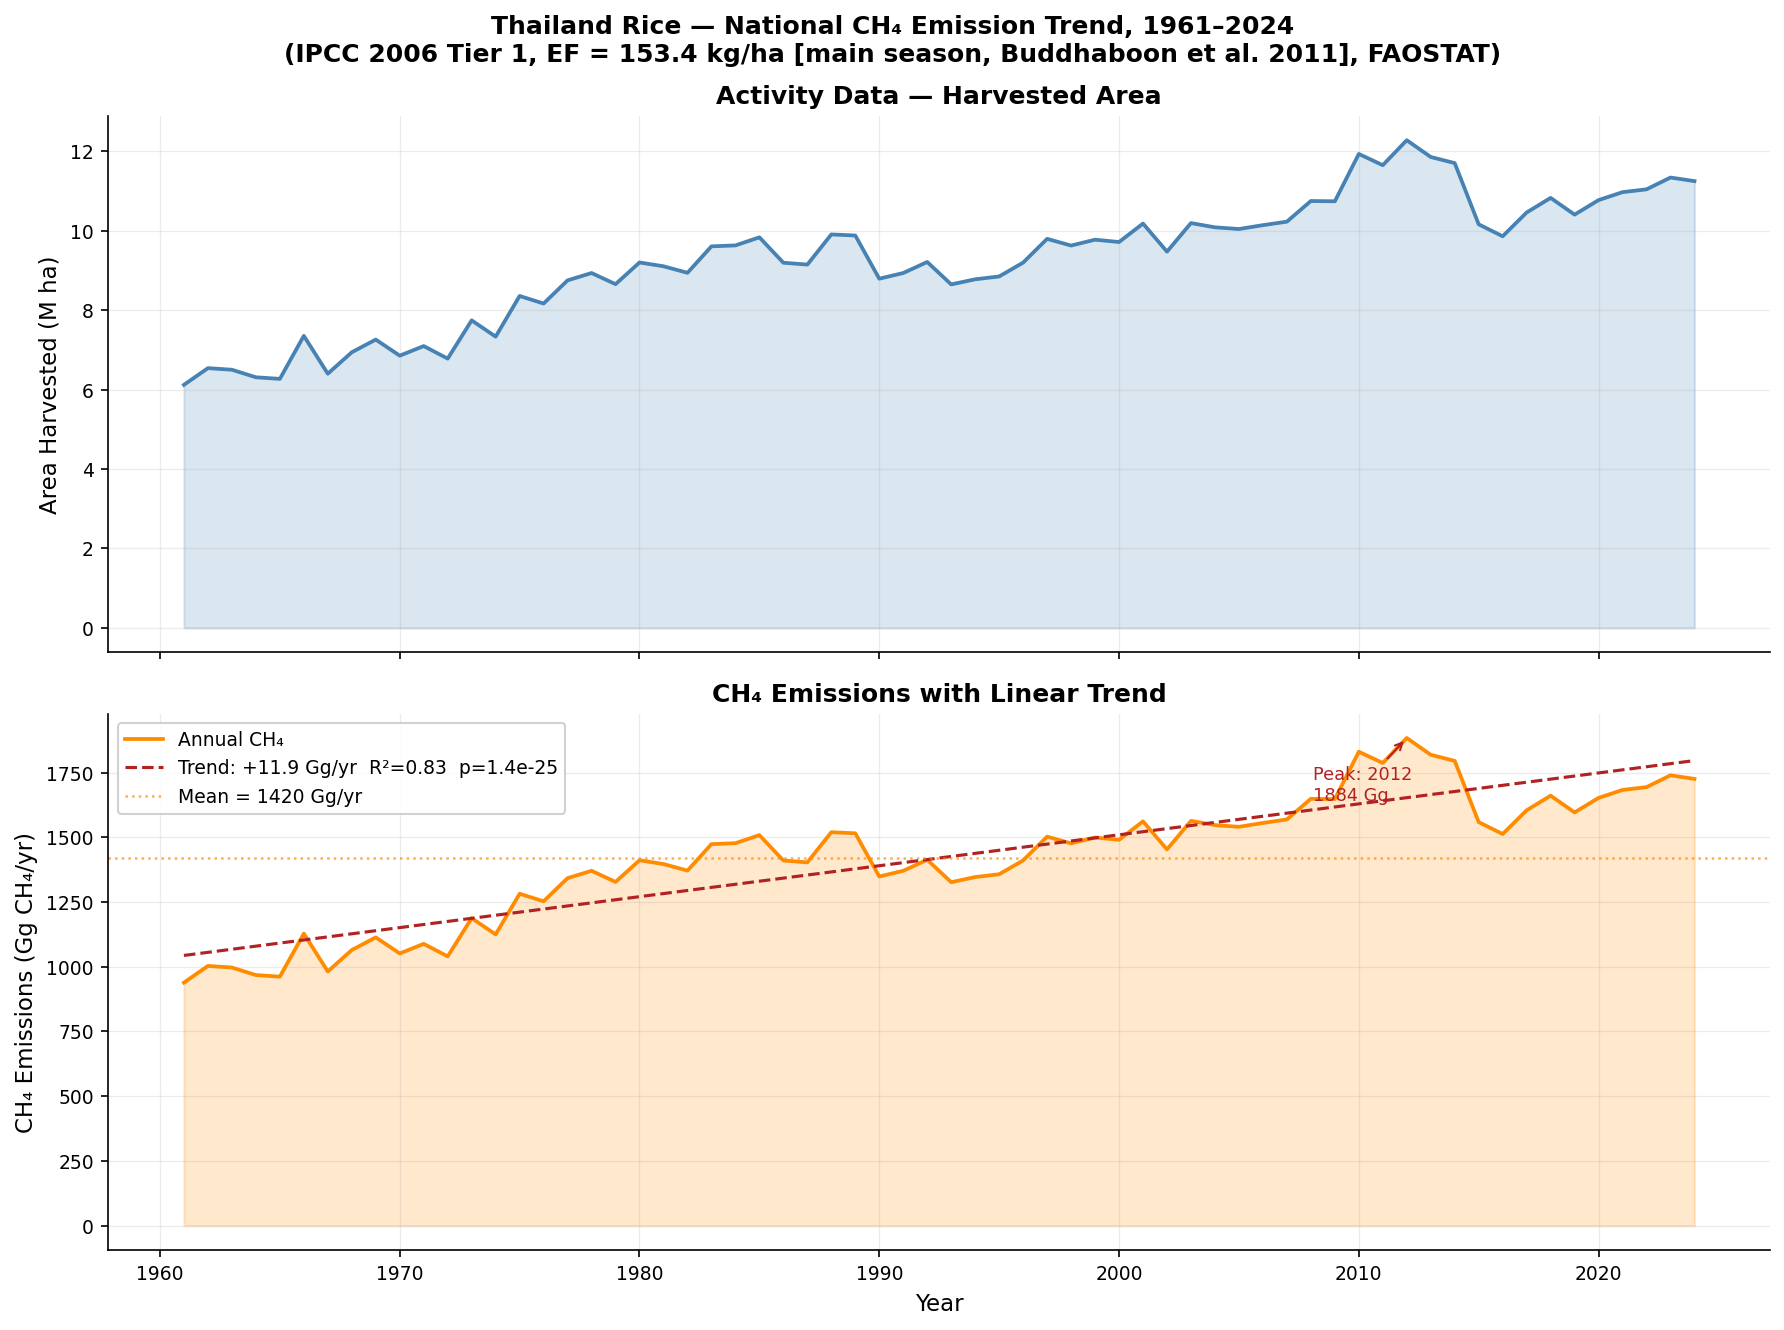
\includegraphics[width=0.96\linewidth]{plot1_national_trend.png}
\caption{National trends in Thailand rice cultivation, 1961--2024.
         \textbf{Top}: Total harvested area (M~ha).
         \textbf{Bottom}: CH\textsubscript{4} emissions
         (Gg~CH\textsubscript{4}~yr\textsuperscript{-1}) with linear trend
         (dashed red) and long-term mean (dotted).
         Source: \cite{faostat2026}; IPCC 2006 Tier~1; authors' calculation.}
\label{fig:national}
\end{figure}

Over the full study period, Thailand's mean annual rice CH\textsubscript{4}
emission was \textbf{1,420~Gg~CH\textsubscript{4}~yr\textsuperscript{-1}}
(39.8~Mt~CO\textsubscript{2}e).
Linear regression reveals a statistically significant upward trend of
\textbf{+12.0~Gg~CH\textsubscript{4}~yr\textsuperscript{-1}}
($R^2 = 0.830$, $p = 1.4 \times 10^{-25}$), confirming that emissions
have risen substantially over six decades.
Emissions grew from 939~Gg in 1961 to a peak of \textbf{1,884~Gg in 2012}
(an increase of 101\%), before declining to 1,726~Gg by 2024.
The 2024 value (48.3~Mt~CO\textsubscript{2}e) represents approximately 13\%
of Thailand's total national GHG emissions, based on the \textasciitilde{}375~Mt~CO\textsubscript{2}e
total reported in Thailand's Third Biennial Update Report \citep{tgo2022}.

The long-run growth reflects two overlapping forces.
From the 1960s through the 1980s, government investment in irrigation
infrastructure and the adoption of high-yielding varieties under Thailand's
Green Revolution allowed farmers to cultivate more land and add a second crop
per year in irrigated areas.
From the 1990s onward, rising global export demand created a sustained
incentive to expand production, as Thailand competed with Vietnam and other
regional exporters for world market share.
Together, these forces drove a steady climb in harvested area and, because
CH\textsubscript{4} scales directly with flooded area under Tier~1, in
emissions.
The 2012 peak stands apart: it was not driven by these long-run structural
forces but by a government scheme that made unlimited area expansion
immediately profitable (discussed below).

Despite rising absolute emissions, Thailand's emission intensity (CH\textsubscript{4}
per tonne of rice produced) has declined sharply over six decades
(Figure~\ref{fig:efficiency}).
Intensity fell from \textbf{92.5~kg~CH\textsubscript{4}~t\textsuperscript{-1}}
in 1961 to \textbf{51.4~kg~CH\textsubscript{4}~t\textsuperscript{-1}} in 2024,
a reduction of 44\%, with a highly significant downward trend of
$-0.730$~kg~t\textsuperscript{-1}~yr\textsuperscript{-1}
($R^2 = 0.892$, $p < 0.001$).

\begin{figure}[!htbp]
\centering
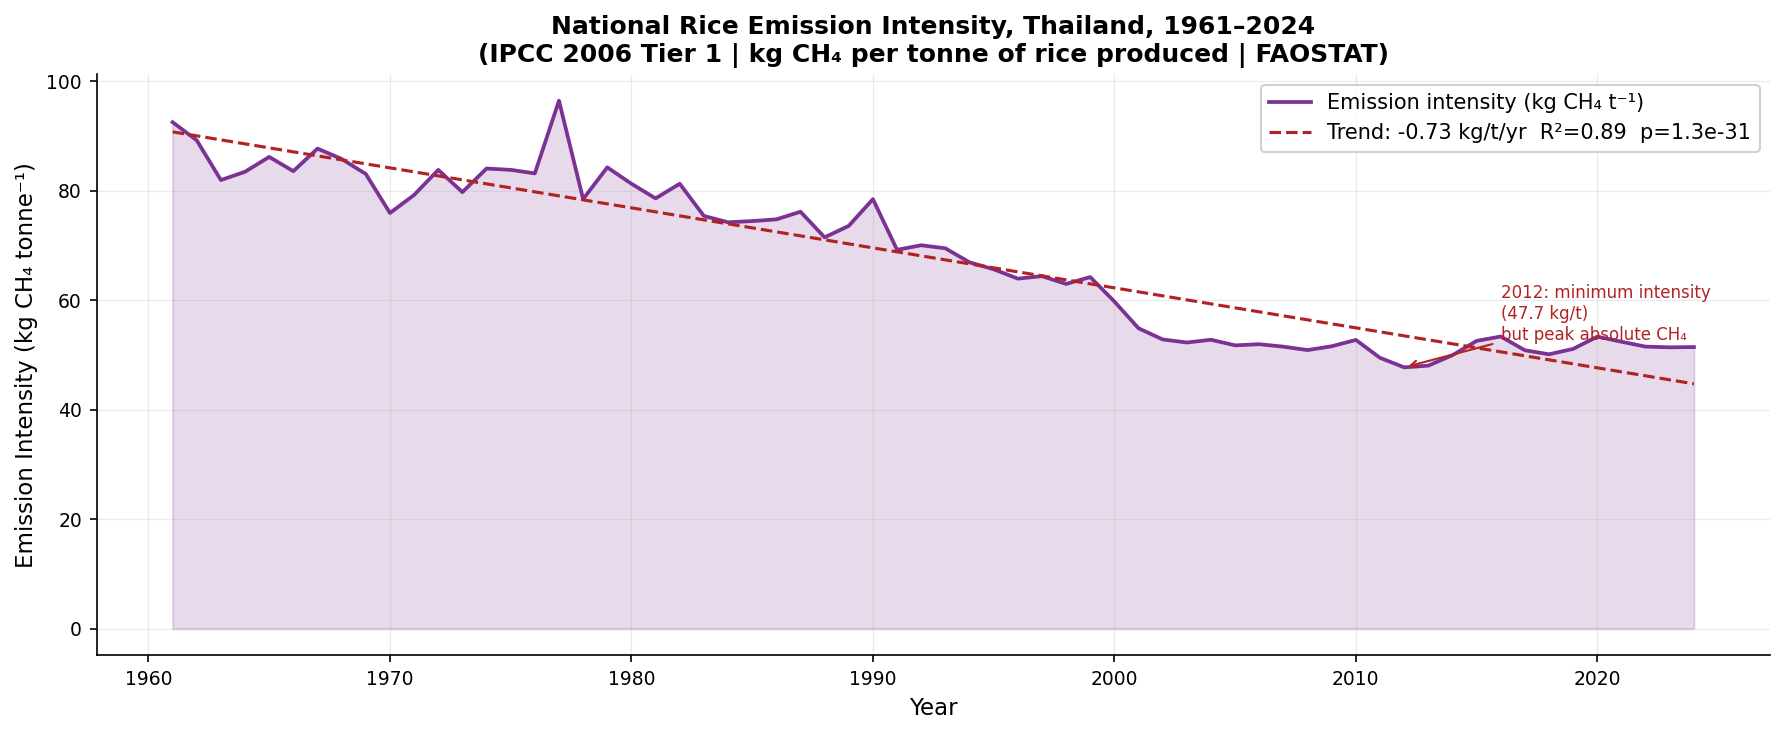
\includegraphics[width=0.96\linewidth]{plot8_yield_efficiency.png}
\caption{National rice emission intensity (kg~CH\textsubscript{4} per tonne
         of rice produced), Thailand, 1961--2024, with linear trend (dashed red).
         Intensity has declined 44\% over six decades as yield growth outpaced
         area expansion.
         Source: \cite{faostat2026}; IPCC 2006 Tier~1; authors' calculation.}
\label{fig:efficiency}
\end{figure}

This is a real \textbf{food-system efficiency gain}: Thailand now produces
each tonne of rice at 44\% lower climate cost than in 1961.
The improvement reflects nationwide adoption of improved seed varieties
and expanded irrigation, which raised average yields across all regions.
Irrigated areas, particularly the Central Plains double-crop system,
contributed disproportionately high yields, pulling the national average up
and reducing the CH\textsubscript{4} cost per tonne of rice produced.
It does \textbf{not} mean less methane per hectare.
Under Tier~1, intensity is simply $\text{EF}_c \times t_p$ divided by yield, so the
decline is automatic when yields rise, not a sign of improved field-level water
management.
Whether actual CH\textsubscript{4} flux per hectare has changed requires Tier~2 field
measurements to detect.
Finally, total emissions still rose 84\% over the same period, because farmers planted
more land faster than yields improved.
The minimum intensity year was \textbf{2012} (47.7~kg~t\textsuperscript{-1}):
the Pledging Scheme's output incentive drove yields to record levels in
Central irrigated areas, inadvertently producing Thailand's most food-efficient
harvest on a per-tonne basis, the same year absolute emissions peaked.

This juxtaposition reveals a critical paradox for climate policy: \textbf{yield
improvement and absolute emission reduction do not automatically co-occur}.
Under Tier~1, higher yield reduces emission intensity mechanically (the same
CH\textsubscript{4} is spread over more tonnes of rice), but leaves absolute
emissions entirely unchanged: only area matters.
Beyond the accounting identity, yield gains can actively \textit{increase}
absolute emissions through a rebound effect: more profitable production per
hectare raises the return to planting, attracting more farmers and pushing
marginal land into cultivation.
Thailand's 64-year record illustrates this precisely: the Green Revolution
raised both yields \textit{and} planted area simultaneously, so absolute
emissions climbed even as intensity fell.
The implication for policy is direct: programmes that raise on-farm yields
without constraining area (through caps, zoning, or purchase limits) may
inadvertently drive emission increases.
Yield improvement reduces absolute CH\textsubscript{4} only if it enables
the \textit{same total production on less land}, a land-sparing outcome that
requires deliberate area management, not just better agronomy.

\FloatBarrier
\subsection*{Spatial distribution of the climate cost}

Figure~\ref{fig:choropleth} maps mean annual CH\textsubscript{4} emissions
per province for 2022--2024.
The Northeast clearly dominates the spatial pattern, consistent with its
large paddy area on the Khorat Plateau.

\begin{figure}[!htbp]
\centering
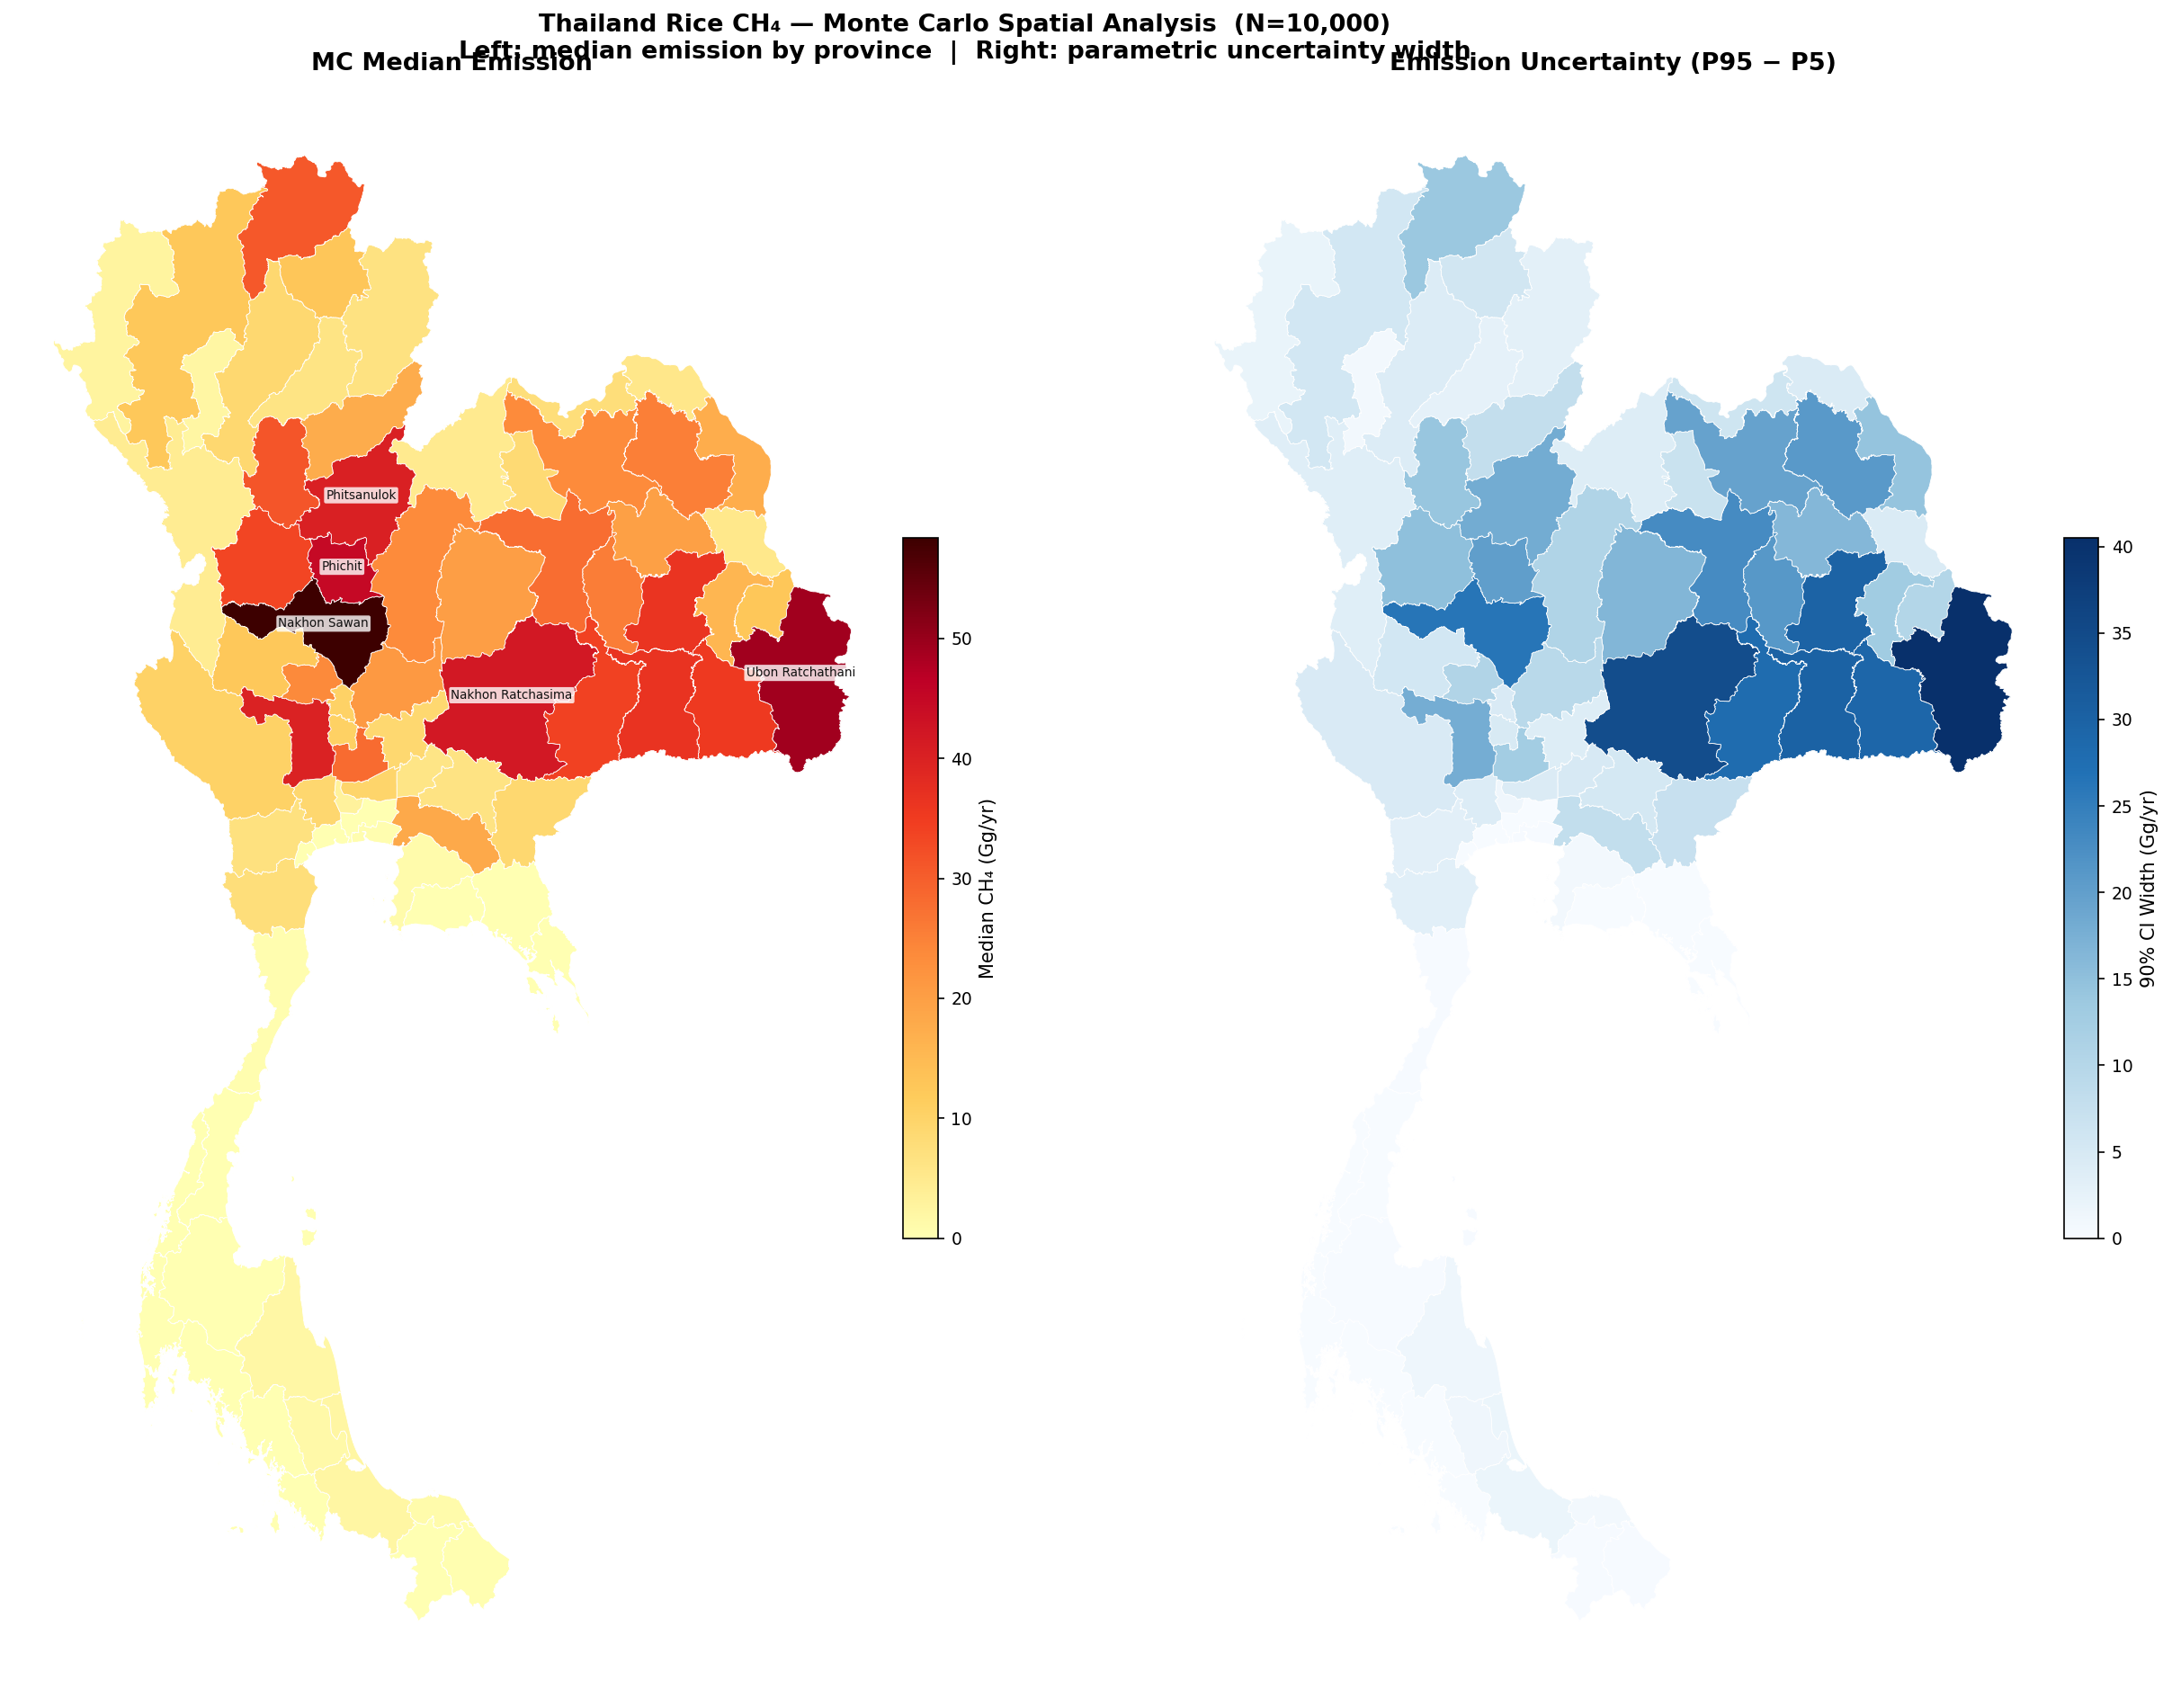
\includegraphics[width=0.98\linewidth]{plot4_choropleth_mc.png}
\caption{Monte Carlo spatial analysis of mean annual rice CH\textsubscript{4} emissions
         by province, Thailand, 2022--2024 ($N = 10{,}000$).
         \textbf{Left:} MC median emission (Gg~yr\textsuperscript{-1}); pale yellow = low,
         near-black = high; top-5 emitting provinces labelled.
         \textbf{Right:} 90\% CI width (P95 $-$ P5), reflecting parametric uncertainty
         from $\text{SF}_w$ and $t_p$; deep blue = highest absolute uncertainty.
         Large irrigated provinces (Central core, North) show the widest CI because
         SF$_w$ variance scales with emission magnitude.
         Source: \cite{oae2024}; \cite{gadm2024}; authors' calculation.}
\label{fig:choropleth}
\end{figure}

\begin{table}[!htbp]
\centering
\caption{Top 10 rice-CH\textsubscript{4}-emitting provinces, Thailand,
         mean annual 2022--2024 (IPCC 2006 Tier~1; $\text{SF}_w$ differentiated:
         0.52 rainfed NE/South, 1.0 irrigated Central/North).}
\label{tab:top10}
\begin{tabular}{@{}clcrrr@{}}
\toprule
\textbf{Rk} & \textbf{Province} & \textbf{Region} &
  \textbf{Area (kha)} &
  \textbf{CH\textsubscript{4} (Gg~yr\textsuperscript{-1})} &
  \textbf{Intensity (kg~t\textsuperscript{-1})} \\
\midrule
1  & Nakhon Sawan           & Central   & 478 &  72.4 & 40.5 \\
2  & Phichit                & North     & 368 &  55.7 & 39.4 \\
3  & Ubon Ratchathani       & Northeast & 662 &  52.7 & 34.7 \\
4  & Phitsanulok            & North     & 331 &  49.9 & 40.2 \\
5  & Suphan Buri            & Central   & 331 &  49.6 & 33.6 \\
6  & Nakhon Ratchasima      & Northeast & 564 &  44.9 & 32.8 \\
7  & Surin                  & Northeast & 491 &  39.1 & 33.2 \\
8  & Roi Et                 & Northeast & 490 &  38.9 & 34.7 \\
9  & Sukhothai              & North     & 258 &  38.9 & 42.2 \\
10 & Chiang Rai             & North     & 253 &  38.3 & 42.6 \\
\bottomrule
\multicolumn{6}{@{}l@{}}{\footnotesize kha = thousand ha; intensity = kg CH\textsubscript{4} per tonne rice produced.}
\end{tabular}
\end{table}

Table~\ref{tab:top10} lists the ten highest-emitting provinces under the
$\text{SF}_w$-differentiated calculation.
\textbf{Nakhon Sawan} (Central, 72.4~Gg~yr\textsuperscript{-1}) now leads,
reflecting its large double-cropped irrigated area (SF$_w$ = 1.0) and high yields.
\textbf{Phichit} (North, 55.7~Gg) ranks second for the same reason.
\textbf{Ubon Ratchathani} (Northeast, 52.7~Gg) falls to third: despite having
the largest cultivated area in the country (662~kha), its rainfed regime
(SF$_w$ = 0.52) halves the per-hectare emission factor.
Nakhon Sawan's position as the top emitter is robust: its 90\% CI spans only ranks 1--3 across all
$N = 10{,}000$ draws, because its irrigated area is large enough that no plausible SF$_w$ draw
allows another province to displace it consistently.

After SF$_w$ differentiation and province-level overrides, the Northeast accounts
for \textbf{40.1\%} (482.0~Gg), while the Central Plains (\textbf{31.3\%},
376.1~Gg) and North (\textbf{27.4\%}, 329.9~Gg) together account for 58.7\%.
The South contributes 1.2\% (14.0~Gg).
Regional SF$_w$ defaults follow IPCC Table~5.12 (0.52 rainfed NE/South; 1.0
irrigated Central/North), with nine peripheral provinces overridden to SF$_w$
= 0.52: the eastern-Central provinces of Sa~Kaeo, Chanthaburi, Trat, Prachin
Buri, Rayong, Chon Buri, and Nakhon Nayok (outside the Chao Phraya irrigation
network), and the remote northern provinces of Mae Hong Son and Tak (highland
mountain rice).
The main wet season dominates emissions in all regions; the dry season
contributes a larger-than-expected share in the Central Plains, where
year-round irrigation supports a second rice crop
(seasonal breakdown in Appendix Figure~\ref{fig:region} and Table~\ref{tab:region}).

\begin{figure}[!htbp]
\centering
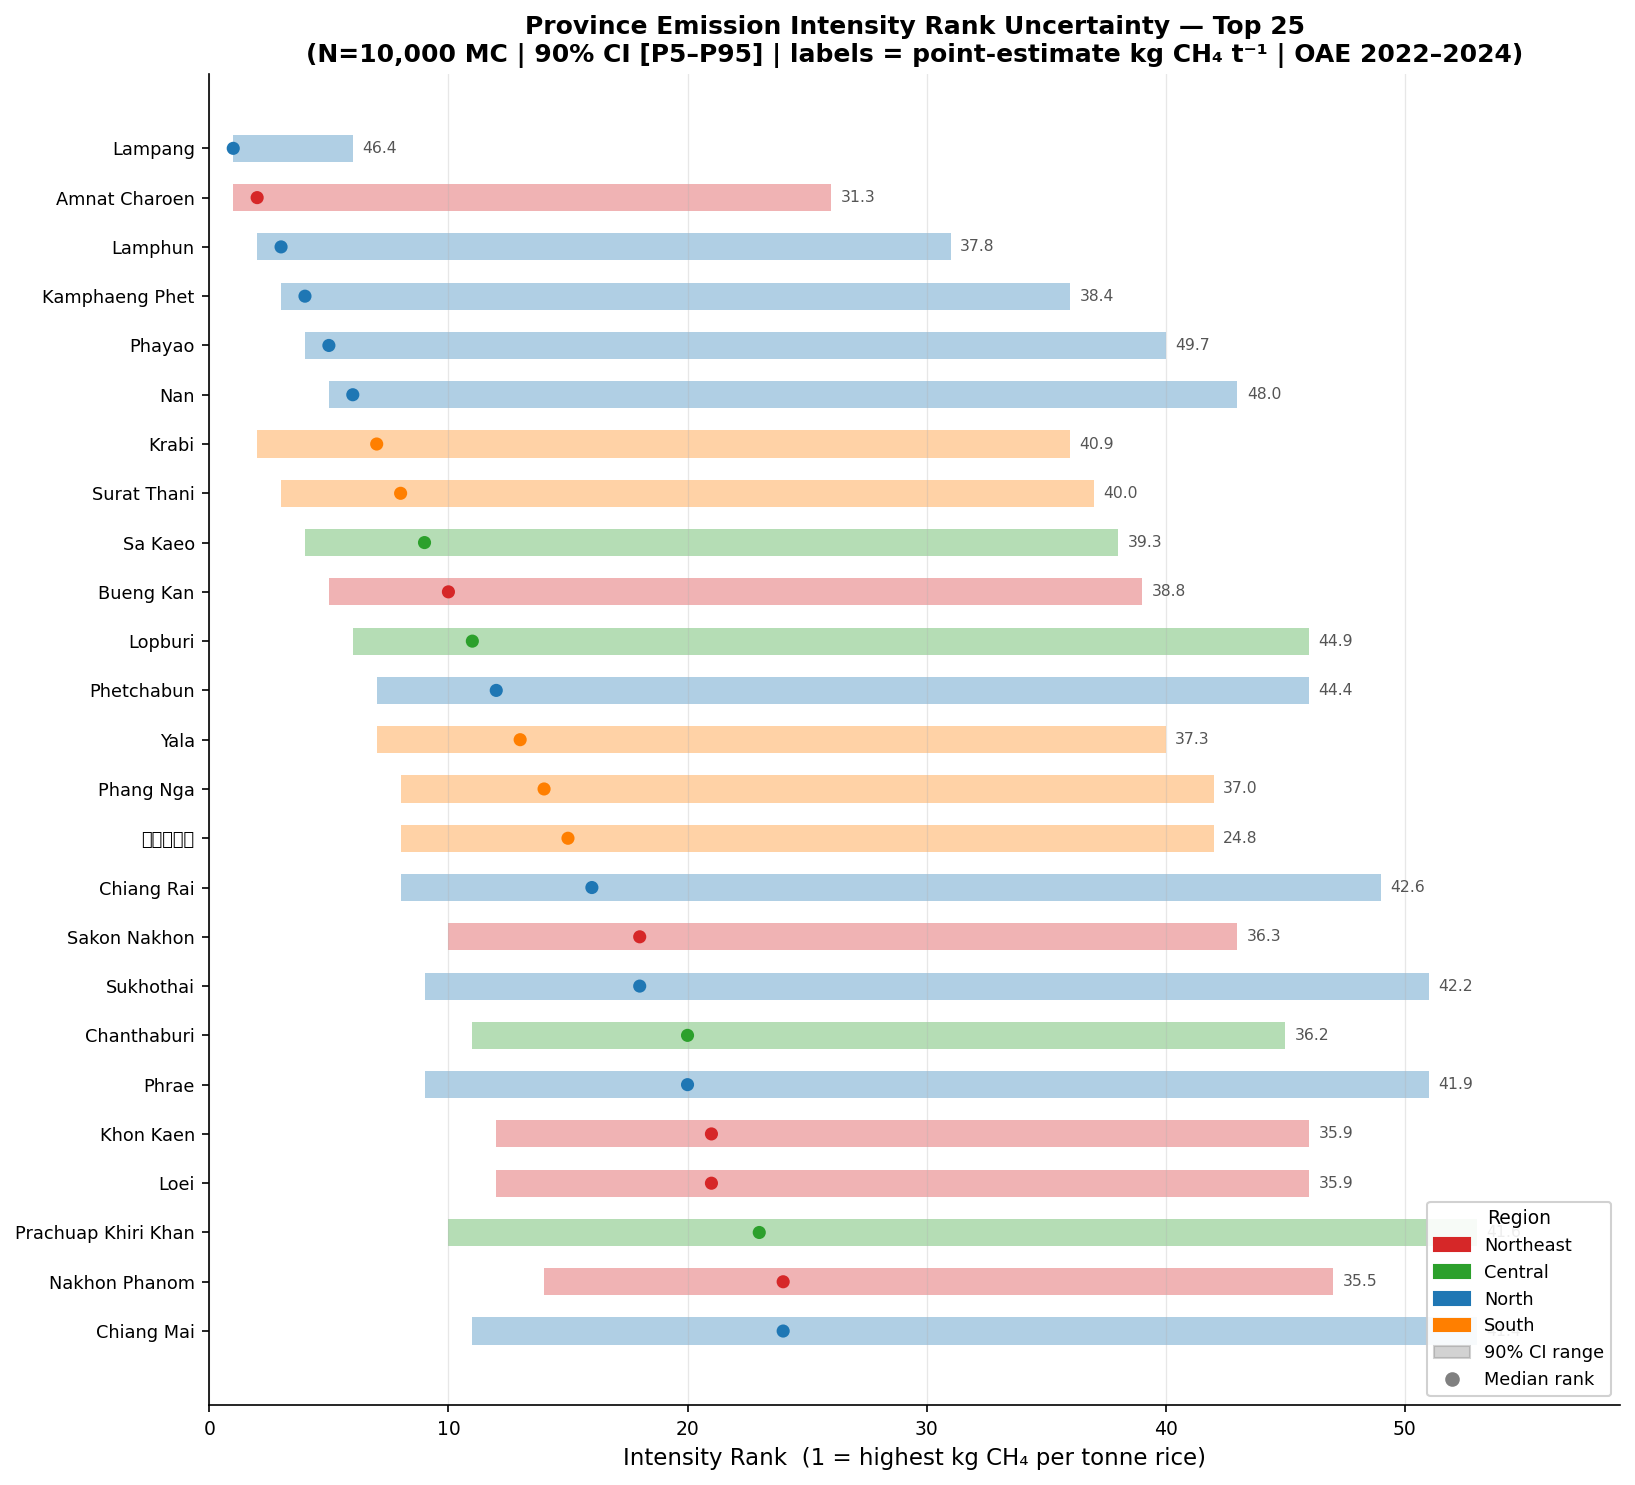
\includegraphics[width=0.82\linewidth]{plot5_intensity_rank.png}
\caption{Top 25 provinces ranked by emission intensity
         (kg~CH\textsubscript{4}~t\textsuperscript{-1} rice produced), with
         Monte Carlo rank uncertainty ($N = 10{,}000$).
         Bars show 90\% CI [P5--P95] of intensity rank; dots show median rank
         (rank 1 = highest intensity).
         Labels give point-estimate intensity.
         Wide CIs reflect sensitivity to the rainfed/irrigated SF$_w$ ratio:
         the intensity ranking is less stable than the absolute-emission ranking
         because the rainfed--irrigated yield differential interacts with the
         SF$_w$ draw to reshuffle province order.
         Source: \cite{oae2024}; authors' calculation.}
\label{fig:intensity}
\end{figure}

Figure~\ref{fig:intensity} reveals a striking reversal from the total-emission
picture once water-regime differences are properly accounted for.
The Northeast dominates national CH\textsubscript{4} \textit{by volume}
(40.1\%, 482~Gg), yet its mean emission intensity
(\textbf{34.0~kg~t\textsuperscript{-1}}) is nearly identical to the Central
Plains (\textbf{34.1~kg~t\textsuperscript{-1}}).
Both trail the \textbf{North} (\textbf{41.0~kg~t\textsuperscript{-1}}), which
carries the highest regional intensity.

The mechanism is clear in the top of the intensity chart: the leading provinces
are all single-crop irrigated North provinces---\textbf{Phayao}
(49.7~kg~t\textsuperscript{-1}), \textbf{Nan} (48.0), \textbf{Lampang}
(46.4)---that receive SF$_w$ = 1.0 (continuously flooded) but produce only one
harvest per year.
Their per-hectare CH\textsubscript{4} flux is high (SF$_w$ = 1.0 × EF$_c$ ×
$t_p$), yet their single-season yield base is modest; the ratio is therefore
higher than in Central double-crop provinces (e.g.\ Nakhon Sawan: 40.5~kg~t\textsuperscript{-1}),
where two harvests per year spread the same per-hectare cost across twice the
production.
The convergence of NE and Central intensity ($\approx$34~kg~t\textsuperscript{-1})
is a direct consequence of correcting SF$_w$: rainfed NE paddies emit half as
much CH\textsubscript{4} per hectare as irrigated Central paddies, and this
reduction exactly offsets the NE yield disadvantage at the regional average.

In short: \textbf{volume and efficiency tell different stories, and both matter
for policy.}
The Northeast is the \textit{quantity} target (largest absolute emissions);
the irrigated North is the \textit{efficiency} target (highest CH\textsubscript{4}
per tonne of rice produced).
These spatial patterns, however, are not fixed: price policy can drive
sharp year-to-year swings in cultivated area and thus total emissions.

\FloatBarrier
\subsection*{Econometrics: price policy as an emission driver}

Geography explains \textit{where} Thailand's rice emissions come from;
price policy explains \textit{when} they spike.
Figure~\ref{fig:policy} overlays farm-gate paddy price, yield, and estimated
CH\textsubscript{4} emissions from 2007 to 2024, annotated with key policy
events; the co-movement between price and CH\textsubscript{4} is immediate and striking.

\begin{figure}[!htbp]
\centering
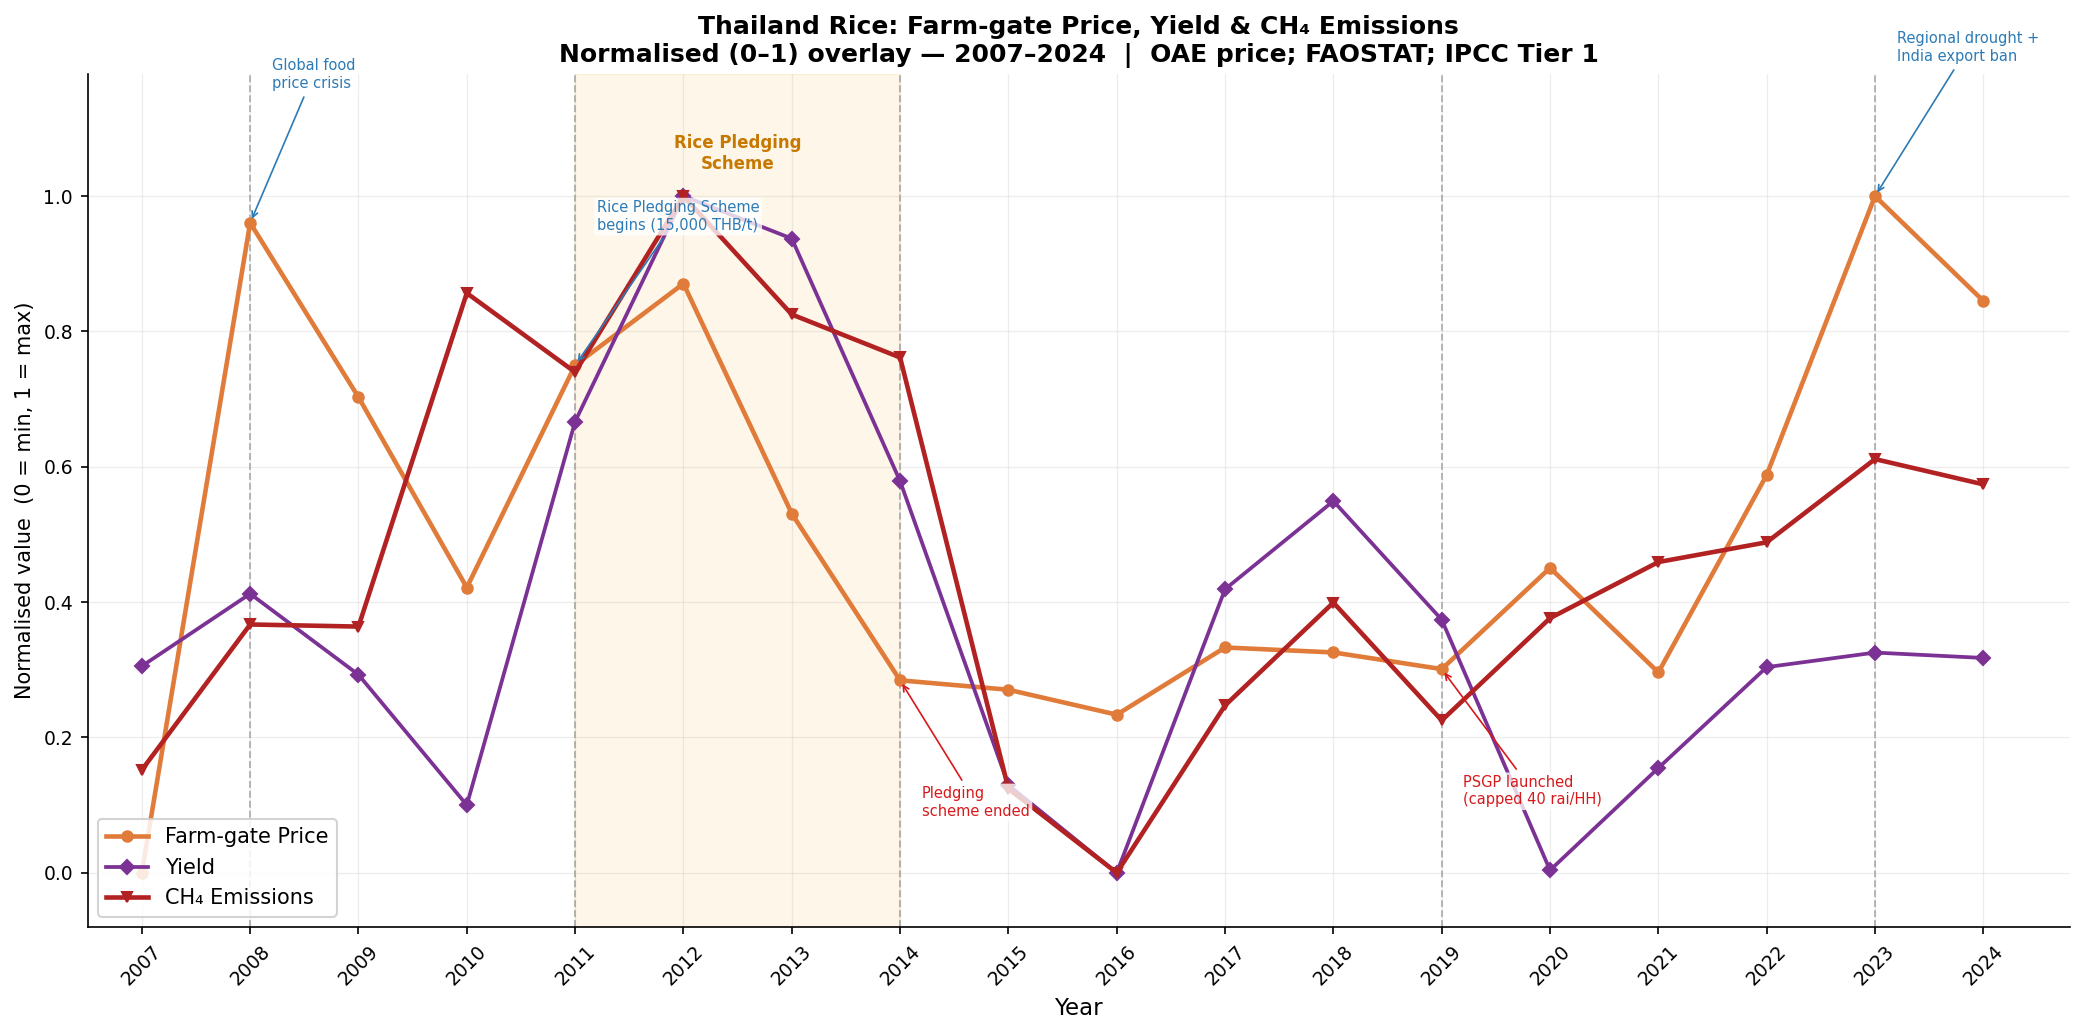
\includegraphics[width=0.96\linewidth]{plot6_policy_timeline.png}
\caption{Thailand rice farm-gate price (THB~tonne\textsuperscript{-1}),
         yield (hg~ha\textsuperscript{-1}), and estimated CH\textsubscript{4}
         emissions (Gg~yr\textsuperscript{-1}), normalised (0--1), 2007--2024.
         Vertical dashed lines mark major policy events.
         Sources: \cite{oae2024} (price); \cite{faostat2026}; authors' calculation.}
\label{fig:policy}
\end{figure}

The price time series shows three distinct periods.
During \textbf{2008}, the global food price crisis briefly doubled farm-gate
prices (6,600 to 10,500~THB~tonne\textsuperscript{-1}), triggering a modest
area expansion.
The most pronounced episode is the \textbf{Rice Pledging Scheme}
(\textit{khrongkan rap chamnam khao}; 2011--2014), introduced as an electoral
commitment by the Pheu Thai government.
The scheme obliged the government to purchase \textit{all} paddy offered by
farmers at 15,000~THB~tonne\textsuperscript{-1} for white rice and
20,000~THB~tonne\textsuperscript{-1} for jasmine, approximately 40--50\%
above world market prices, with \textbf{no quantity cap per
household} \citep{poapongsakorn2014}.
This design created an unlimited expansion incentive: every additional tonne
planted was guaranteed to be profitable regardless of market conditions.
Farmers responded rationally by converting non-rice land to paddy, expanding
double-cropping in irrigated areas, and pushing marginal fields into production.
National harvested area reached record levels and CH\textsubscript{4} reached
its 64-year peak of \textbf{1,884~Gg in 2012}.

The scheme ultimately became fiscally unsustainable.
The government purchased approximately 52\% of total national paddy production
but could not resell stockpiles on world markets: Thai offer prices were too
high relative to competing exporters \citep{usda2017}.
Warehoused rice deteriorated, widespread corruption in storage contracts
emerged, and the total programme cost reached \textbf{984~billion~THB}
(approximately USD~32~billion), equivalent to 41\% of the 2013 national
budget \citep{poapongsakorn2014, usda2017}.
Following the May 2014 military coup, the incoming government cancelled the
scheme; farm-gate prices fell sharply and harvested area contracted by over
5\% in 2014/15, pulling CH\textsubscript{4} downward proportionally.
This sequence---policy introduced, emissions spike, policy cancelled, emissions
fall---is consistent with a causal interpretation, though formal proof would
require a counterfactual comparison region or a more complete model.

Since 2015, the government has operated a lighter-touch \textbf{Price Subsidy
Guarantee Programme} (PSGP), which pays farmers the difference between a
reference price and the market price, capped at 40~rai (6.4~ha) per household.
This redesign shows a key principle: \textit{how} a price-support programme
is structured matters as much as the price level itself.
The Pledging Scheme's unlimited guarantee made every extra hectare profitable
no matter what, a direct incentive to expand.
The PSGP's per-household cap removes that incentive beyond 6.4~ha, limiting
the land-expansion response.
Since 2019, price and area trajectories have been more stable, showing that
climate-friendly policy design does not require abandoning farmer income support.

\FloatBarrier
\subsection*{The counterfactual: emission costs of uncapped guarantees}

\textbf{Counterfactual: the emission cost of programme design.}
The regression dummy coefficient ($\hat{\beta}_2 = 988$~kha) isolates the
structural expansion effect of the unlimited guarantee, the excess area beyond
what the contemporaneous farm-gate price alone would predict.
This provides a direct basis for a counterfactual: \textit{had the Pledging
Scheme included the same 40-rai (6.4~ha) per-household cap as the current PSGP,
this structural expansion would have been constrained.}
Applying the main-season emission factor, the estimated \textbf{avoided
CH\textsubscript{4} is 151.6~Gg~yr\textsuperscript{-1}}, equivalent to 10.7\%
of the long-run national mean, for each year the cap would have been in effect.
Summed across the scheme's four-year duration (2011--2014), the cap would have
prevented approximately \textbf{606~Gg~CH\textsubscript{4}} (17.0~Mt~CO\textsubscript{2}e).
These findings indicate that the structural design of price-support programmes
operates at a scale of emission impact that field-level mitigation technologies
alone are unlikely to match.
The SF$_w$ and season-length uncertainty propagated through the MC does not affect
this figure, since the counterfactual is computed from the national area regression
using the fixed Tier~1 EF.
The counterfactual should be read as an illustrative upper-bound estimate, not
a reliable point estimate, for three reasons.
First, the dummy coefficient ($\hat{\beta}_2 = 988$~kha, $n = 18$) is estimated
from a short time series with omitted variables (rainfall, export demand, input
costs) that are correlated with both price and the scheme dummy; the true
structural expansion effect could be considerably smaller or larger.
Second, the cap would bind only for households already operating above 6.4~ha;
smallholders below that threshold would be unaffected and their price-driven
expansion would continue.
Third, capped subsidy schemes in Thailand have documented instances of
land-title subdivision, where households divide holdings among family members
to remain under the cap threshold, a behavioural response that would partially
erode the cap's effectiveness in practice \citep{poapongsakorn2014}.
The 2023 spike in price (10,700~THB~tonne\textsuperscript{-1}) reflects
regional drought reducing supply combined with elevated
global export demand following the India rice export ban.

Statistical analysis confirms a \textbf{significant positive relationship}
between farm-gate price and harvested area ($r = 0.505$, $p = 0.033$, $n = 18$).
A regression slope of 0.045~Gg~CH\textsubscript{4} per THB~tonne\textsuperscript{-1}
(derived from the area--price slope of 291~ha per THB~tonne\textsuperscript{-1})
implies that a 1,000~THB~tonne\textsuperscript{-1} sustained price increase
is associated with approximately 45~Gg additional CH\textsubscript{4}~yr\textsuperscript{-1},
equivalent to about 2.6\% of the 2024 national total.

\begin{table}[!htbp]
\centering
\caption{Regression of national harvested area on price and Pledging Scheme
         dummy, Thailand, 2007--2024 ($n = 18$). Dependent variable: national
         harvested area (ha). $D_t = 1$ for 2011--2014, 0 otherwise.
         HAC standard errors use Newey--West estimator (maxlags = 1)
         \citep{neweywest1987}.}
\label{tab:dummy}
\begin{tabular}{@{}lrrr@{}}
\toprule
 & \textbf{Model 1} & \textbf{Model 2} & \textbf{Model 2 (HAC)} \\
 & \textit{Price only} & \textit{Price + dummy} & \textit{NW SE} \\
\midrule
Intercept      & 8{,}490{,}000 ha & 8{,}869{,}000 ha & 8{,}869{,}000 ha \\
Price ($\hat{\beta}_1$, ha/THB~t\textsuperscript{-1}) & 291 & 222 & 222 \\
\quad $p$-value            & 0.033 & 0.029 & \textbf{0.005} \\
Pledging dummy ($\hat{\beta}_2$, kha) & --- & $+$988 & $+$988 \\
\quad $p$-value            & --- & 0.001 & \textbf{$<$0.001} \\
\midrule
$R^2$                       & 0.255 & 0.631 & --- \\
$\Delta R^2$                & ---   & $+$0.376 & --- \\
Durbin--Watson              & 1.162 & 2.141 & --- \\
\bottomrule
\multicolumn{4}{@{}l@{}}{\footnotesize CH\textsubscript{4} equivalent of $\hat{\beta}_2$: 151.6~Gg~yr\textsuperscript{-1} (EF = 153.4~kg~ha\textsuperscript{-1}, \citealt{buddhaboon2011}).} \\
\multicolumn{4}{@{}l@{}}{\footnotesize DW $\approx$ 2 for Model~2 indicates autocorrelation resolved once dummy is included.}
\end{tabular}
\end{table}

To test whether the Pledging Scheme expanded area beyond the price effect
alone, a policy dummy ($D_t = 1$ for 2011--2014) was added to the regression
(Equation~\ref{eq:dummy}; Table~\ref{tab:dummy}).
Adding the dummy raises $R^2$ from 0.255 to 0.631.
The dummy coefficient ($\hat{\beta}_2 = 988$~kha) shows that the Pledging
Scheme years are linked to roughly \textbf{988,000 additional hectares}
beyond what price alone explains, equivalent to
\textbf{151.6~Gg~CH\textsubscript{4}~yr\textsuperscript{-1}}
(4,245~Gg~CO\textsubscript{2}e).
The price slope also drops from 291 to 222~ha per THB~tonne\textsuperscript{-1}
once the dummy is included, showing the simpler model was blending the
scheme's direct area effect with the general price response.
Both effects remain highly significant under Newey--West HAC standard errors
\citep{neweywest1987} ($p_{\text{price}} = 0.005$;
$p_{\text{pledging}} < 0.001$).
The dummy coefficient should be read as capturing the scheme's \textit{combined}
effect (both the price premium and the structural guarantee of unlimited
government purchasing) rather than a clean separation of the two, given that
$D_t$ and $P_t$ are correlated during the 2011--2014 pledge years.

\FloatBarrier
\subsection*{Forward-looking mitigation: targeting AWD in irrigated systems}

\begin{figure}[!htbp]
\centering
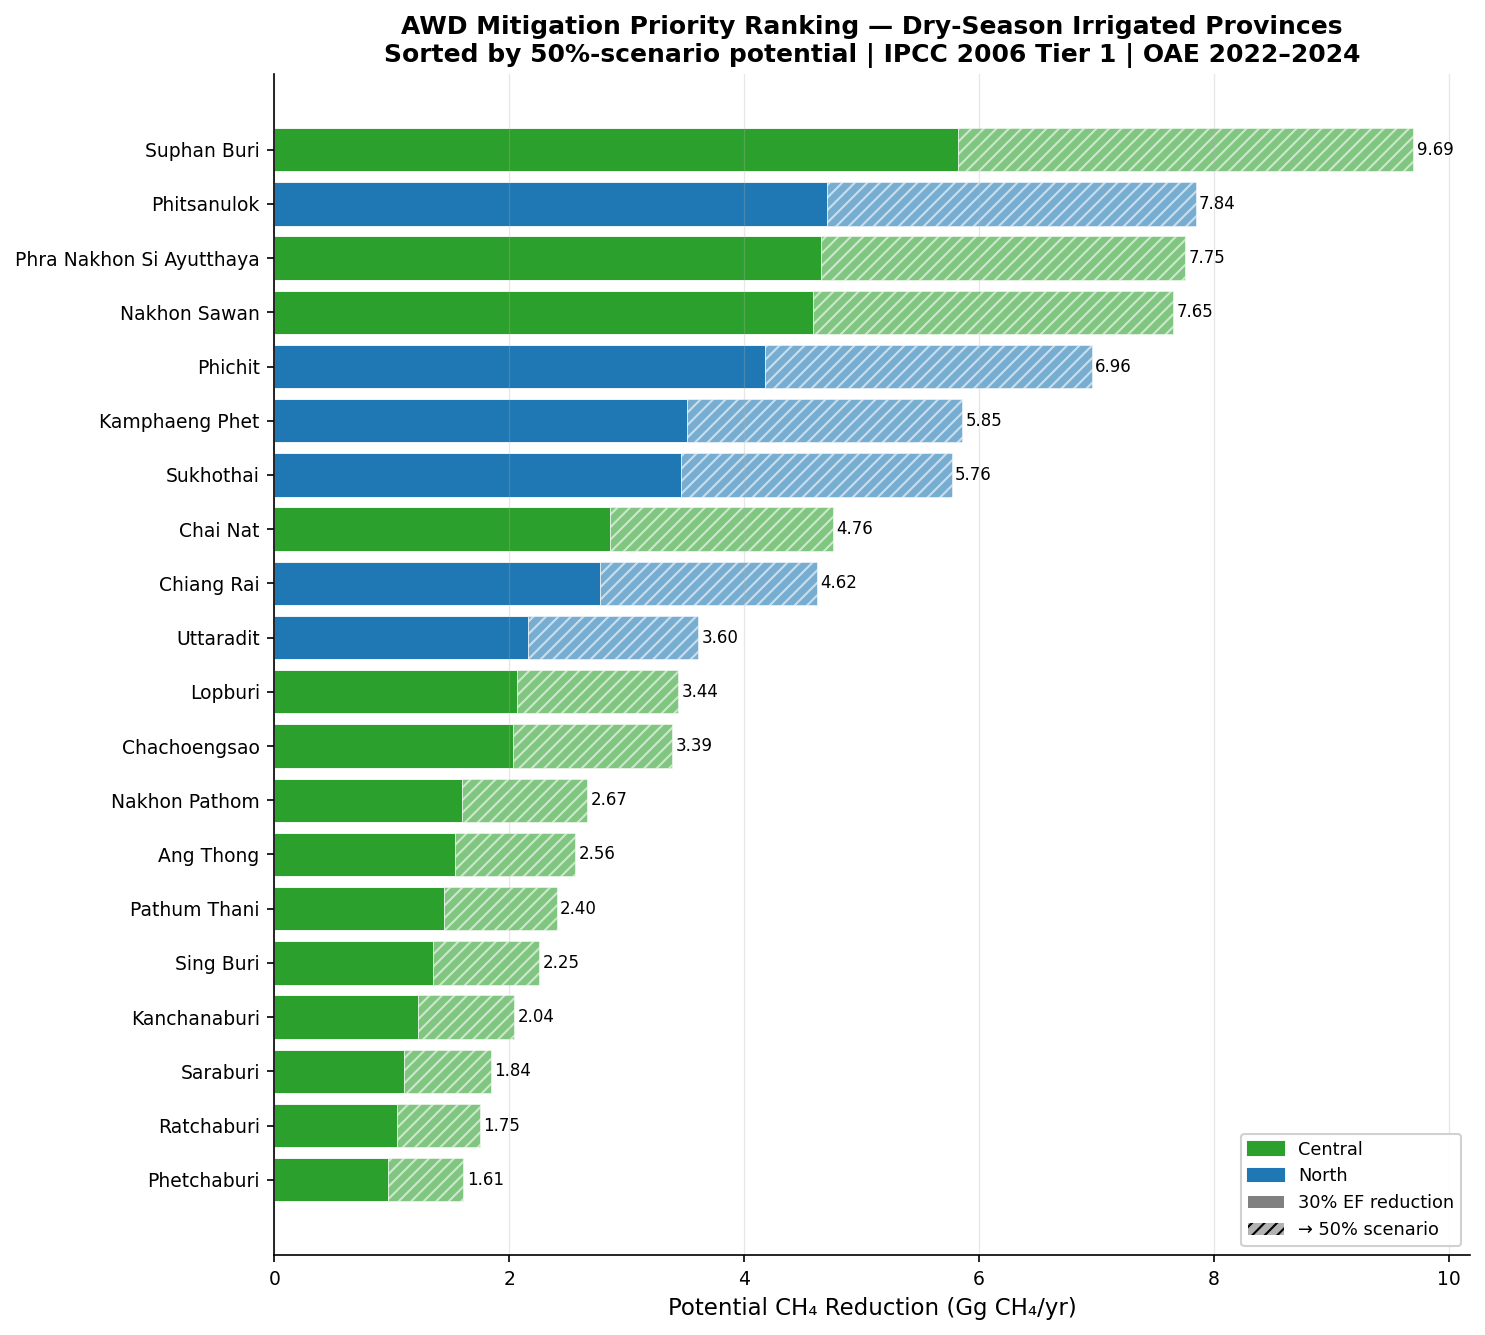
\includegraphics[width=0.96\linewidth]{plot9_awd_priority.png}
\caption{AWD mitigation priority ranking by province.
         Bars show potential CH\textsubscript{4} reduction under 30\% (solid)
         and 50\% (hatched extension) EF reduction scenarios applied to
         dry-season irrigated area only.
         Bar colour indicates macro-region.
         Source: \cite{oae2024}; authors' calculation.}
\label{fig:awd}
\end{figure}

These findings have direct policy implications.
First, \textbf{price-support programmes must account for their emission
co-effects}: purchasing guarantees that raise farm-gate prices above equilibrium
will expand the cultivated area and increase CH\textsubscript{4} proportionally.
Emission impact assessments should be a standard component of rice subsidy
design under Thailand's NDC framework.
Second, \textbf{targeted adoption of Alternate Wetting and Drying (AWD)},
which involves intermittent drainage during the growing season, could cut per-hectare CH\textsubscript{4}
by 30--50\% without yield loss \citep{wassmann2000, maneepitak2019, sriphirom2023}.
A suitability assessment across six Central Thai provinces (Ang Thong, Ayutthaya,
Chai Nat, Pathum Thani, Sing Buri, and Suphan Buri) estimated annual CH\textsubscript{4}
reductions of 32\% under AWD adoption---24\% in the major wet season and 41\%
in the dry season \citep{prangbang2020}.
AWD is applicable only to the dry-season irrigated area, where water control
infrastructure enables scheduled drainage; only 25\% of Thailand's rice area
is irrigated \citep{ccac2021}, limiting AWD's national reach to the Central
and North provinces.
Province-level analysis of dry-season harvested area (Figure~\ref{fig:awd})
identifies \textbf{Suphan Buri} (Central), \textbf{Phitsanulok} (North),
\textbf{Phra Nakhon Si Ayutthaya} (Central), and \textbf{Nakhon Sawan} (Central)
as the highest-priority provinces, together accounting for
35\% of national AWD mitigation potential.
Applying a conservative 30\% EF reduction to irrigated dry-season provinces yields
a national reduction of \textbf{57.3~Gg~yr\textsuperscript{-1}}
(3.3\% of the 2024 total); a 50\% reduction saves \textbf{95.5~Gg~yr\textsuperscript{-1}}
(5.5\%).
Extending AWD incentives through carbon credit mechanisms tied to Thailand's NDC
represents a priority opportunity \citep{thailand_ndc2022}.
Critically, Thailand's evolving price-support architecture offers a direct
implementation lever: embedding AWD compliance as a prerequisite for PSGP subsidy
payments would align income transfers with climate outcomes, delivering
CH\textsubscript{4} reductions precisely in the irrigated areas where water
control is feasible and programme monitoring is most practicable.

Four concrete policy steps follow from this analysis.
First, AWD adoption should be \textbf{prioritised} in Suphan Buri, Phitsanulok,
Phra Nakhon Si Ayutthaya, and Nakhon Sawan, the four provinces that together
account for the largest share of national AWD mitigation potential and already
operate the irrigation infrastructure required for scheduled drainage.
Second, AWD compliance should be made a \textbf{mandatory condition} for
PSGP subsidy receipt rather than a voluntary option, using OAE's existing
plot-level monitoring to verify adoption without creating a parallel
bureaucracy.
Third, verified AWD emission reductions should be linked to Thailand's
\textbf{domestic carbon market} or international climate finance instruments
under the NDC framework \citep{thailand_ndc2022}, giving irrigated-area
farmers a direct monetary incentive that complements the income guarantee.
Together, these steps would use the same PSGP administrative architecture
that already caps area expansion to additionally mandate cleaner water
management, turning a single programme into a dual lever for income support
and climate compliance.
Fourth, the \textbf{North} carries the highest emission intensity
(41.0~kg~t\textsuperscript{-1}) because its provinces are single-crop
continuously flooded but produce only one harvest per year.
\textbf{AWD adoption in North irrigated provinces} therefore addresses both the
efficiency and absolute emission dimensions simultaneously---cutting the
per-hectare CH\textsubscript{4} flux while maintaining yield.
For the Northeast, where SF$_w$ = 0.52 already reflects natural drying cycles,
\textbf{drought-tolerant variety programmes} that raise yields would reduce
intensity without requiring changes to water management infrastructure.

\subsection*{Limitations and uncertainties}

The biggest source of uncertainty in this study is probably the water management
assumption.
The provincial analysis assigns SF$_w$ = 0.52 to the Northeast and South rainfed
provinces and SF$_w$ = 1.0 for continuously flooded irrigated conditions (Central
and North)---an improvement over the uniform Tier~1 baseline but still an
approximation.
Under IPCC Table~5.12, 0.52 is the \textit{irrigated} intermittently flooded
factor; the rainfed regular default is 0.28.
Within the Northeast, flooding regimes vary considerably: deeper-flood zones
(e.g.\ the Mun River basin) may sustain near-continuous inundation, while drier
upland rainfed areas are closer to the rainfed regular regime (SF$_w$ = 0.28),
suggesting the true provincial average lies somewhere in the 0.28--0.52 range.
Using a single regional value of 0.52 therefore remains a simplification;
Northeast estimates presented here are best read as regional averages rather
than precise provincial values.
For Central Thailand specifically, field experiments in Ayutthaya found that
AWD irrigation reduces CH\textsubscript{4} by 34--39\% versus continuous
flooding \citep{maneepitak2019}, implying an effective SF$_w$ in the range
0.61--0.66 under water-saving management and suggesting the IPCC default
of 1.0 may overestimate actual Central emissions by 30--40\%.
This uncertainty is captured in the Monte Carlo analysis via a wider
SF$_w$ irrigated range of [0.61, 1.00].
The national time-series estimates (1961--2024) use the standard Tier~1 value
SF$_w$ = 1.0, consistent with national inventory reporting practice, and should
be interpreted as a conservative upper bound.

A more fundamental constraint is the Tier~1 formula itself.
Because CH\textsubscript{4} = EF $\times$ Area and neither the emission factor
nor the scaling factors respond to price signals, any policy-driven area expansion
produces an exactly proportional emission increase by construction.
The observed correlation between price support and emissions is therefore partly
a methodological artifact of the linear inventory formula, not direct evidence of
a real-world biophysical change.
A Tier~2 approach --- in which field-measured EFs vary with actual water management,
organic inputs, and variety choice --- could produce a different relationship if
higher-price years systematically alter management practices (e.g.\ greater fertiliser
use or more intensive flooding to boost yields).
This study's policy conclusions are directionally robust under Tier~1 because the
causal mechanism (price $\rightarrow$ area expansion $\rightarrow$ more flooded
hectares) is real and empirically supported; but the quantitative emission figures
should be understood as inventory constructs rather than independent physical measurements.

The uniform cultivation period (118 days main season, 111 days dry season,
\citealt{buddhaboon2011}) is a second simplification.
Real season lengths vary by province and variety (\citealt{buddhaboon2011} report
$\sigma$ = 5 days for main season and $\sigma$ = 6 days for dry season across varieties
and planting dates), and province-level data to differentiate them remain limited.

To formally propagate the key parametric uncertainties,
Figure~\ref{fig:mc} presents a Monte Carlo analysis ($N = 10{,}000$) varying
four parameters: $\text{SF}_w$ rainfed (uniform, 0.27--0.71),
$\text{SF}_w$ irrigated (uniform, 0.61--1.00), and both season lengths
(normal, $\sigma$ = 5 days main season and $\sigma$ = 6 days dry season,
derived from \citealt{buddhaboon2011} Table~1 across varieties and planting dates).
EF$_c$ is held fixed at the IPCC 2006 Tier~1 default of 1.30~kg~ha\textsuperscript{-1}~day\textsuperscript{-1}
\citep{ipcc2006}; the analysis is designed to quantify uncertainty from the
regional SF$_w$ grouping assumption (two classes for 77 provinces), not from
the emission factor itself.
The lower bound of 0.61 for irrigated SF$_w$ is derived from field experiments
in Ayutthaya, Central Thailand, where AWD reduced CH\textsubscript{4} by
34--39\% versus continuous flooding \citep{maneepitak2019}, while the
upper bound of 1.00 retains the IPCC default for continuously flooded conditions.

\begin{figure}[!htbp]
\centering
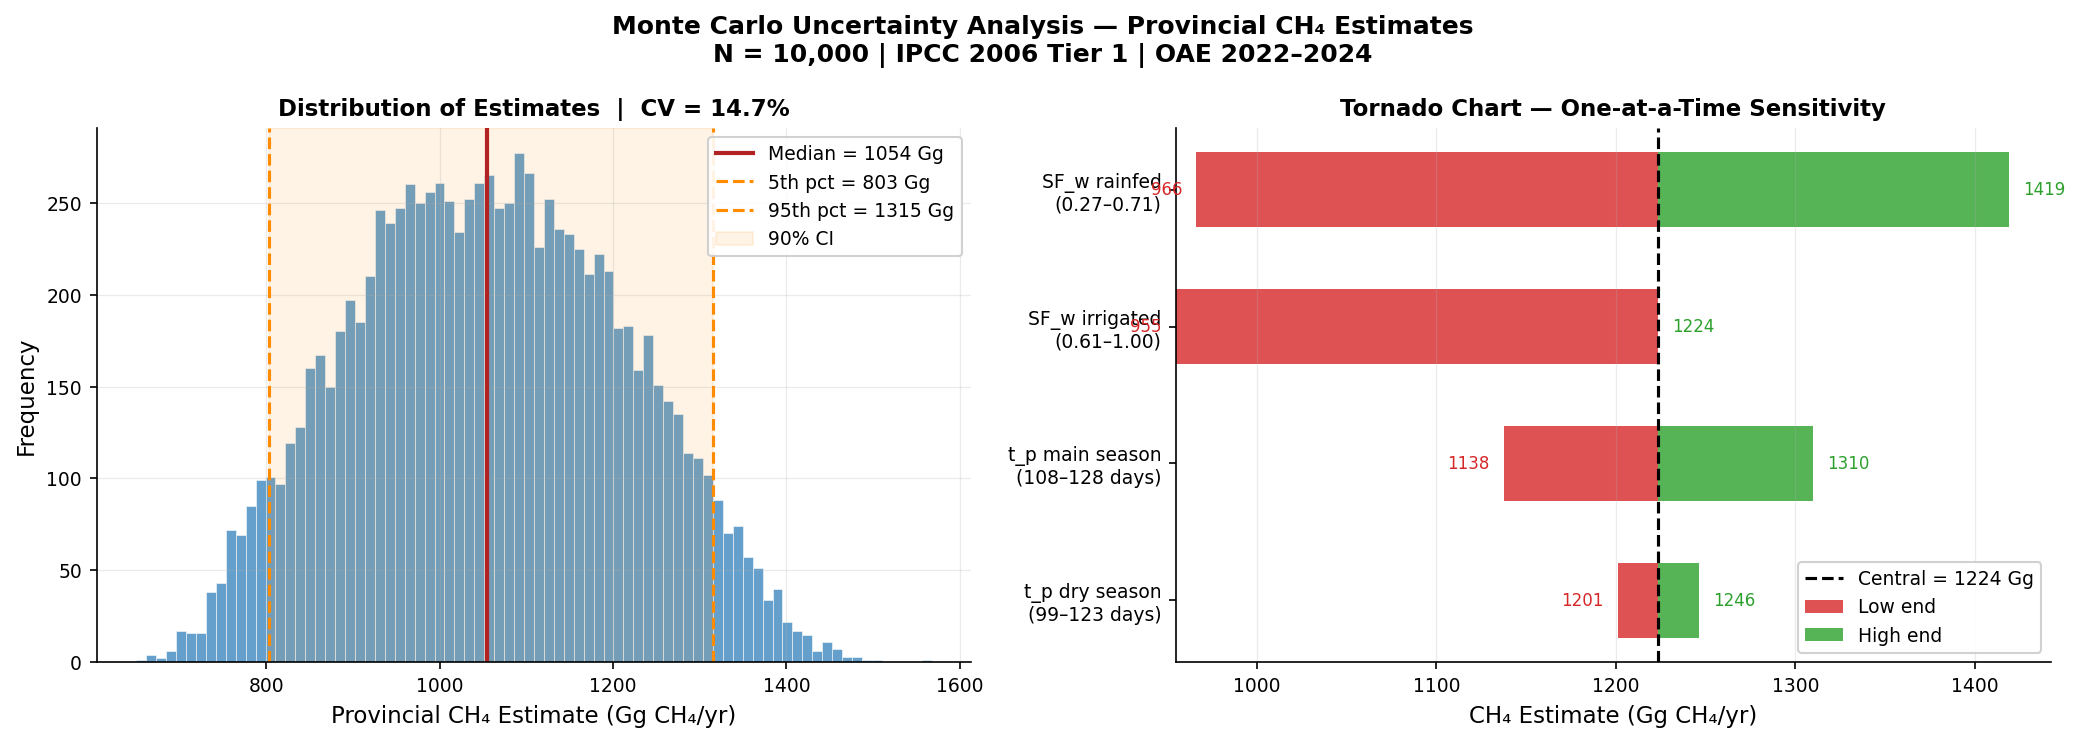
\includegraphics[width=0.96\linewidth]{plot_mc_uncertainty.png}
\caption{Monte Carlo uncertainty analysis ($N = 10{,}000$) for provincial
         CH\textsubscript{4} estimates. \textit{Left:} distribution of
         simulated totals; median = 1,054~Gg, 90\% CI [803, 1{,}315]~Gg,
         CV = 14.7\%. \textit{Right:} tornado chart — one-at-a-time sensitivity
         showing SF$_w$ rainfed as the dominant source of uncertainty, confirming
         that the regional water-regime classification drives model output more
         than season length. EF$_c$ is fixed at the IPCC Tier~1 default (1.30).
         Irrigated SF$_w$ lower bound [0.61] from \citet{maneepitak2019};
         upper bound 1.00 is the IPCC default.
         Source: authors' calculation; IPCC 2006 \citep{ipcc2006}.}
\label{fig:mc}
\end{figure}

With EF$_c$ fixed, the distribution is near-symmetric with a coefficient of
variation of \textbf{14.7\%}, substantially tighter than the $\sim$50\% uncertainty
reported in global rice CH\textsubscript{4} inventories that also vary EF$_c$
\citep{yan2009}.
This 14.7\% CV reflects \textit{classification uncertainty only} --- the uncertainty
in SF$_w$ regional grouping and season length --- and should not be interpreted as
total inventory uncertainty; allowing EF$_c$ to vary over its published range
would raise the CV to approximately 45--50\% \citep{yan2009}.
The tornado chart confirms that \textbf{SF$_w$ rainfed dominates}
(966--1,419~Gg), because 43 of 77 provinces draw from the rainfed
uniform distribution and the NE accounts for 40\% of total area.
Main-season length is second (1,136--1,308~Gg), irrigated SF$_w$ is third
(955--1,224~Gg), and dry-season length contributes negligibly (1,199--1,244~Gg).
This hierarchy directly validates the analytical focus of this paper:
the largest reducible uncertainty is the two-class SF$_w$ grouping; replacing it
with province-specific flooding-regime data (Tier~2) would narrow the CI more
than any other methodological improvement.
The policy conclusions are unaffected by this uncertainty: the trend direction,
the Pledging Scheme significance ($p < 0.001$), and regional emission shares
are derived from area data and regression slopes and do not depend on SF$_w$.
Province-level emission \textit{ranks} carry additional uncertainty beyond the
aggregate total: because EF$_c$ and $t_p$ scale all provinces identically, only
the rainfed/irrigated SF$_w$ ratio can reshuffle the rank order.
A province-level Monte Carlo (same $N = 10{,}000$ draws, applied as a $76 \times N$
emission matrix) shows that \textbf{Nakhon Sawan}'s top rank is stable (90\% CI:
ranks 1--3), while mid-table Northeast and North provinces may shift by 10--20
positions.

Field-measured, province-specific emission factors would address the Tier~1
uncertainties on the methods side \citep{wassmann2000, yan2009}.
A natural extension is a province-level Tier~2 study applying
field-measured $\text{SF}_w$ values rather than the regional categorical
defaults used here.
Such a study would replace the two-class (0.52/1.0) approximation with
province-specific flooding-regime data, further refining the spatial pattern.
Under Tier~2, provinces at the wetter end of the NE distribution (deeper-flood
areas) might see SF$_w$ approach 0.8--1.0, while drier upland rainfed areas
could be as low as 0.28.
Crucially, the North and Central Plains---identified here as the highest-intensity
irrigated regions (SF$_w$ = 1.0, North intensity 41.0~kg~t\textsuperscript{-1})---would
retain elevated SF$_w$ values under Tier~2, validating the AWD priority ranking
derived in this study.
Finally, while the policy section proposes embedding AWD compliance as a
condition for PSGP subsidy receipt, implementing this credibly requires
monitoring infrastructure beyond what currently exists: scheduled drainage
must be documented through water-level sensors, soil moisture records, or
sufficiently high-resolution remote sensing, none of which OAE's current
plot-area surveys provide.
MRV build-out costs should therefore be evaluated against mitigation benefits
before mandatory conditionality is adopted.

% =============================================================
\section*{Conclusions}
% =============================================================

Thai rice paddies are a significant and growing source of agricultural
methane, but one whose trajectory is shaped more by the structural design
of price-support programmes than by either agronomic improvement or
field-level mitigation technology.
The central finding of this study is that a single design choice (the absence
of a per-household area cap in the 2011--2014 Rice Pledging Scheme) is
estimated to have generated 606~Gg~CH\textsubscript{4} (17.0~Mt~CO\textsubscript{2}e)
of avoidable emissions over four years --- an upper-bound estimate illustrating
the emission leverage of programme-design decisions.
The practical implication is that Thailand's path to meeting its NDC
agriculture targets runs primarily through the design of its next rice
price-support programme, not through yield improvement or AWD alone.
The key findings of this study are:

\begin{enumerate}[noitemsep]
  \item National emissions increased significantly at +12.0~Gg~yr\textsuperscript{-1}
        ($R^2 = 0.830$, $p < 0.001$) over 1961--2024, peaking at 1,884~Gg in 2012
        and reaching 1,726~Gg (48.3~Mt~CO\textsubscript{2}e) in 2024.

  \item Applying IPCC Table~5.12 $\text{SF}_w$ with province-level overrides
        for nine peripheral rainfed provinces, the Northeast accounts for
        40.1\% (482.0~Gg~yr\textsuperscript{-1}), Central 31.3\% (376.1~Gg),
        and North 27.4\% (329.9~Gg); \textbf{Nakhon Sawan} (Central, 72.4~Gg)
        is the highest-emitting single province.
        A Monte Carlo uncertainty analysis ($N = 10{,}000$) yields a 90\% CI of
        [803, 1{,}315]~Gg for the provincial total, with CV = 14.7\%;
        SF$_w$ rainfed is the dominant uncertainty driver, confirming that
        province-level water-regime classification is the binding methodological constraint.

  \item National emission intensity declined from 92.5 to 51.4~kg~CH\textsubscript{4}~t\textsuperscript{-1}
        ($-$44\%; $R^2 = 0.892$, $p < 0.001$), reflecting a genuine food-system efficiency gain
        as yield growth outpaced area expansion.
        This is \textit{relative} decoupling only: absolute emissions rose 84\% over the
        same period, and per-hectare flux is unchanged under Tier~1's constant EF.

  \item   After SF$_w$ correction with province-level overrides, the \textbf{North}
        carries the highest mean intensity (41.0~kg~CH\textsubscript{4}~t\textsuperscript{-1}),
        driven by single-crop irrigated provinces; the Central Plains and
        Northeast converge at $\approx$34~kg~t\textsuperscript{-1} once
        eastern-Central rainfed provinces are correctly reclassified (SF$_w$
        = 0.52).
        AWD targets irrigated provinces where SF$_w$ = 1.0 elevates
        per-hectare flux.

  \item Farm-gate price is a significant positive predictor of harvested area
        ($r = 0.505$, $p = 0.033$, $n = 18$); the 2011--2014 Rice Pledging Scheme
        added $\sim$988,000~ha beyond the price effect alone, consistent with a
        policy-induced area expansion driving the 2012 emission peak.

  \item \textbf{Programme design determines emission risk more than price level.}
        A counterfactual cap-equivalent calculation estimates that a 40-rai
        per-household limit applied from 2011 would have avoided
        \textbf{606~Gg~CH\textsubscript{4}} (17.0~Mt~CO\textsubscript{2}e)
        over the scheme's four-year duration (upper-bound estimate).
        Future price-support programmes should treat area cap design as a
        primary climate-policy variable, not an afterthought.

  \item \textbf{Yield improvement does not automatically reduce absolute emissions.}
        Emission intensity fell 44\% over 1961--2024 as yields improved, yet
        absolute emissions rose 84\% because yield gains raised the profitability
        of rice farming and attracted area expansion (rebound effect).
        The 2012 emission peak coinciding with Thailand's lowest-ever emission
        intensity (47.7~kg~t\textsuperscript{-1}) illustrates this directly.
        Absolute CH\textsubscript{4} reduction requires either area contraction
        or water management change; yield improvement alone is insufficient and
        may be counterproductive when paired with uncapped price guarantees.

  \item AWD adoption across dry-season irrigated provinces reduces national
        CH\textsubscript{4} by 3--6\% under 30--50\% EF reduction scenarios
        (57.3~Gg and 95.5~Gg~yr\textsuperscript{-1} respectively),
        with irrigated Central and North provinces (led by Suphan Buri [Central]
        and Phitsanulok [North]) accounting for the largest share of
        mitigation potential.
        Embedding AWD compliance as a condition for PSGP subsidy receipt
        represents the most actionable mitigation pathway under Thailand's NDC.
\end{enumerate}

% =============================================================
\section*{Acknowledgements}

The authors thank the Food and Agriculture Organization of the United Nations
for FAOSTAT data access, and the Office of Agricultural Economics, Ministry of
Agriculture and Cooperatives, Thailand, for provincial rice statistics and
price data.

% =============================================================
\section*{AI Use Disclosure}

Claude (Anthropic), an AI language model, was used during the preparation of
this manuscript to assist with prose editing, structural feedback, and LaTeX
formatting.
All data collection, emission calculations, statistical analysis, and
intellectual conclusions are the author's own.
The author takes full responsibility for the accuracy and integrity of the
content presented.

% =============================================================
\section*{Appendix}
% =============================================================

\noindent
These appendices document the full provincial dataset and highlight a key divergence
between production volume and emission intensity.
The Northeast dominates rice output ($\sim$14.2~Mt~yr$^{-1}$, 43\% of national production)
but its rainfed water regime (SF$_w$ = 0.52) keeps emission intensity at
$\approx$34~kg~CH$_4$~t$^{-1}$---essentially equal to the irrigated Central Plains.
The North achieves the highest intensity (41.0~kg~t$^{-1}$) despite ranking
third in absolute output, because single-crop irrigated systems combine full
flooding (SF$_w$ = 1.0) with moderate yields ($\sim$3.45~t~ha$^{-1}$).
Small North provinces such as Phayao (49.7~kg~t$^{-1}$) and Nan
(48.0~kg~t$^{-1}$) rank among the most emission-intensive but contribute little
to total volume.

% ─── Table A1: Regional summary ───────────────────────────────────────────────
\begin{table}[!htbp]
\centering
\small
\caption{Regional rice CH\textsubscript{4} emission summary, mean annual 2022--2024
         (IPCC 2006 Tier~1, SF$_w$-differentiated; \dag{}~marks provinces with
         rainfed override applied within administrative region).}
\label{tab:region}
\begin{tabular}{@{}lrrrrrrrr@{}}
\toprule
\textbf{Region} &
  \textbf{Provs} &
  \textbf{Area} &
  \textbf{Prod.} &
  \textbf{Yield} &
  \textbf{CH\textsubscript{4}} &
  \textbf{CO\textsubscript{2}e} &
  \textbf{Share} &
  \textbf{Int.} \\
 & & \footnotesize(kha) & \footnotesize(Mt) & \footnotesize(t~ha\textsuperscript{-1}) &
   \footnotesize(Gg) & \footnotesize(Gg) & \footnotesize(\%) &
   \footnotesize(kg~t\textsuperscript{-1}) \\
\midrule
Northeast & 20 & 6,060 & 14.18 & 2.35 &  482.0 & 13,497 & 40.1 & 34.0 \\
Central   & 28 & 2,648 & 10.45 & 3.87 &  376.1 & 10,531 & 31.3 & 34.1 \\
North     & 15 & 2,225 &  8.01 & 3.45 &  329.9 &  9,239 & 27.4 & 41.0 \\
South     & 14 &   178 &  0.54 & 2.61 &   14.0 &    393 &  1.2 & 31.4 \\
\midrule
\textbf{Total} & \textbf{77} & \textbf{11,110} & \textbf{33.16} & --- &
  \textbf{1,202.1} & \textbf{33,660} & \textbf{100.0} & --- \\
\bottomrule
\multicolumn{9}{@{}l@{}}{\footnotesize SF$_w$: NE/South = 0.52; Central/North = 1.0 (IPCC Table 5.12); 9 override provinces = 0.52.}
\end{tabular}
\end{table}

\begin{figure}[!htbp]
\centering
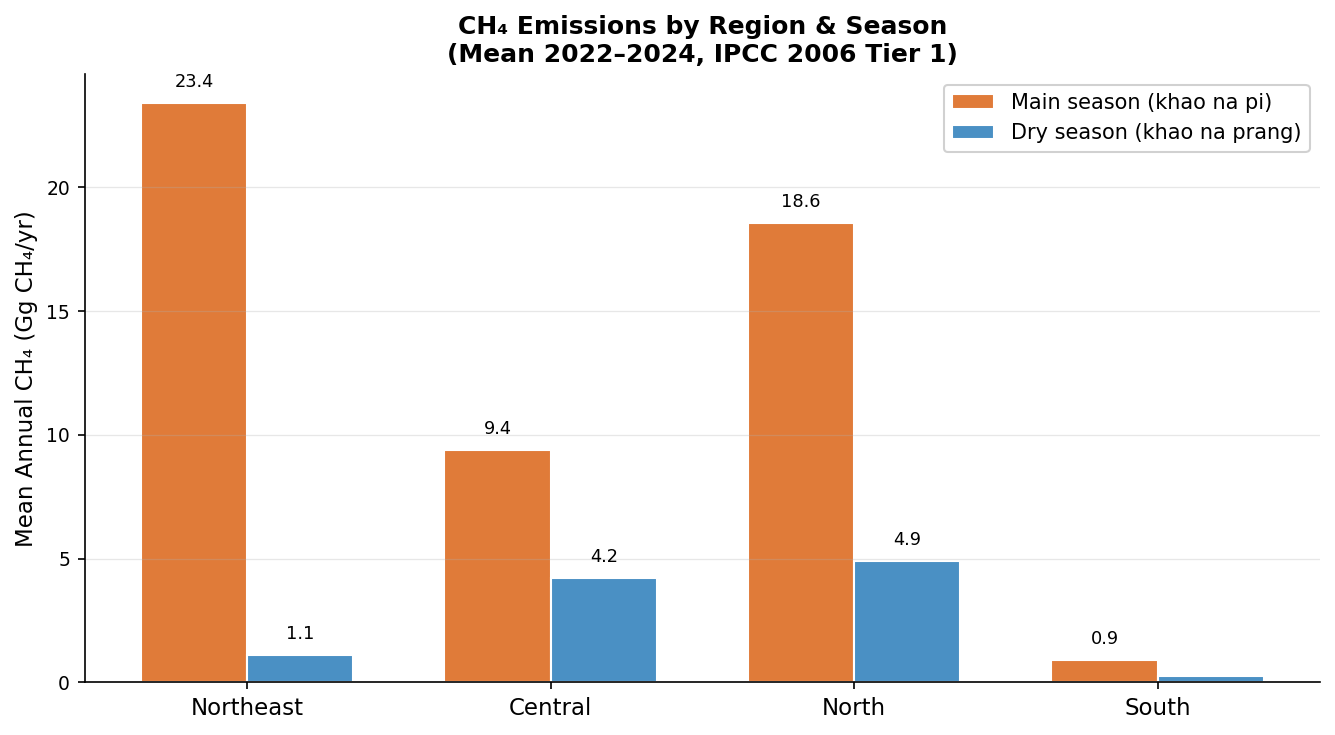
\includegraphics[width=0.92\linewidth]{plot3_region_season.png}
\caption{Mean annual rice CH\textsubscript{4} emissions by region and season,
         Thailand, 2022--2024.
         Orange: main season (\textit{khao na pi});
         blue: dry season (\textit{khao na prang}).
         Source: \cite{oae2024}; authors' calculation.}
\label{fig:region}
\end{figure}

% ─── Table A2: Top 20 by intensity ────────────────────────────────────────────
\FloatBarrier
\begin{table}[H]
\centering
\small
\caption{Top 20 provinces by rice CH\textsubscript{4} emission intensity
         (kg CH\textsubscript{4} per tonne of rice), mean 2022--2024.
         North provinces dominate, driven by irrigated single-crop systems
         (SF$_w$ = 1.0) combined with moderate yields.
         $^*$~Province with rainfed override (SF$_w$ = 0.52 applied despite
         Central/North administrative classification).
         $^\dagger$~Small-area South provinces (\textless{}3~kha); intensity
         estimates unreliable due to sampling noise.}
\label{tab:top20int}
\begin{tabular}{@{}clllrrrr@{}}
\toprule
\textbf{Int.} & \textbf{Province} & \textbf{Region} & \textbf{SF$_w$} &
  \textbf{Yield} & \textbf{CH\textsubscript{4}} & \textbf{Int.} & \textbf{Prod.} \\
\textbf{Rank} & & & &
  \footnotesize(t~ha\textsuperscript{-1}) & \footnotesize(Gg) &
  \footnotesize(kg~t\textsuperscript{-1}) & \textbf{Rank} \\
\midrule
 1 & Phayao           & North     & 1.00 & 3.07 &  15.9 & 49.7 & 35 \\
 2 & Nan              & North     & 1.00 & 3.19 &   8.4 & 48.0 & 47 \\
 3 & Lampang          & North     & 1.00 & 3.23 &   7.7 & 46.4 & 48 \\
 4 & Lopburi          & Central   & 1.00 & 3.36 &  26.1 & 44.9 & 24 \\
 5 & Phetchabun       & North     & 1.00 & 3.45 &  29.2 & 44.4 & 22 \\
 6 & Chiang Rai       & North     & 1.00 & 3.55 &  38.3 & 42.6 & 13 \\
 7 & Sukhothai        & North     & 1.00 & 3.57 &  38.9 & 42.2 & 12 \\
 8 & Phrae            & North     & 1.00 & 3.64 &   7.6 & 41.9 & 46 \\
 9 & Prachuap KK$^b$  & Central   & 1.00 & 3.61 &   0.6 & 41.6 & 62 \\
10 & Chiang Mai       & North     & 1.00 & 3.67 &  15.5 & 41.4 & 30 \\
11 & Krabi$^\dagger$  & South     & 0.52 & 1.95 &   0.1 & 40.9 & 73 \\
12 & Nakhon Sawan     & Central   & 1.00 & 3.74 &  72.4 & 40.5 &  1 \\
13 & Phitsanulok      & North     & 1.00 & 3.75 &  49.9 & 40.2 &  6 \\
14 & Surat Thani$^\dagger$ & South & 0.52 & 1.99 &  0.2 & 40.0 & 68 \\
15 & Phichit          & North     & 1.00 & 3.84 &  55.7 & 39.4 &  4 \\
16 & Sa Kaeo$^*$      & Central   & 0.52 & 2.03 &   9.5 & 39.3 & 44 \\
17 & Uttaradit        & North     & 1.00 & 3.83 &  21.9 & 39.2 & 25 \\
18 & Bueng Kan        & Northeast & 0.52 & 2.05 &   5.9 & 38.8 & 50 \\
19 & Kamphaeng Phet   & North     & 1.00 & 3.87 &  31.6 & 38.4 & 16 \\
20 & Uthai Thani      & Central   & 1.00 & 4.01 &  15.5 & 37.9 & 28 \\
\bottomrule
\multicolumn{8}{@{}l@{}}{\footnotesize $^b$~Prachuap Khiri Khan (abbreviated).}
\end{tabular}
\end{table}

% ─── Table A4: Full provincial inventory ──────────────────────────────────────
\FloatBarrier
\begin{longtable}{@{}rllcrrrr@{}}
\caption{Complete provincial rice CH\textsubscript{4} inventory, mean annual
         2022--2024, IPCC 2006 Tier~1 (76 named administrative units).
         Sorted by CH\textsubscript{4} emissions (descending).
         $^\dagger$~rainfed override province.
         Area and production are two-season totals per province.
         One unattributed OAE South-region aggregate entry (73~kha; 5.75~Gg~CH\textsubscript{4})
         is included in regional totals (Table~A1) but excluded here;
         Phuket province not reported by OAE (negligible rice cultivation).}
\label{tab:all76} \\
\toprule
\textbf{\#} & \textbf{Province} & \textbf{Region} & \textbf{SF$_w$} &
  \textbf{Area} & \textbf{Prod.} & \textbf{CH\textsubscript{4}} &
  \textbf{Int.} \\
 & & & & \footnotesize(kha) & \footnotesize(Mt) &
  \footnotesize(Gg) & \footnotesize(kg~t\textsuperscript{-1}) \\
\midrule
\endfirsthead
\multicolumn{8}{c}{\tablename\ \thetable{} -- continued}\\
\toprule
\textbf{\#} & \textbf{Province} & \textbf{Region} & \textbf{SF$_w$} &
  \textbf{Area} & \textbf{Prod.} & \textbf{CH\textsubscript{4}} &
  \textbf{Int.} \\
 & & & & \footnotesize(kha) & \footnotesize(Mt) &
  \footnotesize(Gg) & \footnotesize(kg~t\textsuperscript{-1}) \\
\midrule
\endhead
\midrule
\multicolumn{8}{r}{\footnotesize Continued on next page\ldots}\\
\endfoot
\bottomrule
\multicolumn{8}{@{}l@{}}{\footnotesize Source: OAE \citep{oae2024}; IPCC 2006 \citep{ipcc2006}; authors' calculation.}
\endlastfoot
 1 & Nakhon Sawan       & Central   & 1.00          & 478 & 1.789 & 72.44 & 40.5 \\
 2 & Phichit            & North     & 1.00          & 368 & 1.412 & 55.66 & 39.4 \\
 3 & Ubon Ratchathani   & Northeast & 0.52          & 662 & 1.519 & 52.71 & 34.7 \\
 4 & Phitsanulok        & North     & 1.00          & 331 & 1.241 & 49.92 & 40.2 \\
 5 & Suphan Buri        & Central   & 1.00          & 331 & 1.476 & 49.59 & 33.6 \\
 6 & Nakhon Ratchasima  & Northeast & 0.52          & 564 & 1.368 & 44.87 & 32.8 \\
 7 & Surin              & Northeast & 0.52          & 491 & 1.177 & 39.10 & 33.2 \\
 8 & Roi Et             & Northeast & 0.52          & 490 & 1.121 & 38.92 & 34.7 \\
 9 & Sukhothai          & North     & 1.00          & 258 & 0.922 & 38.90 & 42.2 \\
10 & Chiang Rai         & North     & 1.00          & 253 & 0.900 & 38.29 & 42.6 \\
11 & Si Sa Ket          & Northeast & 0.52          & 477 & 1.090 & 37.97 & 34.9 \\
12 & Buri Ram           & Northeast & 0.52          & 459 & 1.066 & 36.55 & 34.3 \\
13 & Ayutthaya$^a$      & Central   & 1.00          & 235 & 1.027 & 35.08 & 34.2 \\
14 & Kamphaeng Phet     & North     & 1.00          & 210 & 0.813 & 31.57 & 38.4 \\
15 & Khon Kaen          & Northeast & 0.52          & 376 & 0.833 & 29.91 & 35.9 \\
16 & Chai Nat           & Central   & 1.00          & 197 & 0.780 & 29.59 & 37.9 \\
17 & Phetchabun         & North     & 1.00          & 191 & 0.659 & 29.24 & 44.4 \\
18 & Maha Sarakham      & Northeast & 0.52          & 347 & 0.831 & 27.58 & 33.2 \\
19 & Sakon Nakhon       & Northeast & 0.52          & 343 & 0.752 & 27.29 & 36.3 \\
20 & Lopburi            & Central   & 1.00          & 173 & 0.582 & 26.11 & 44.9 \\
21 & Udon Thani         & Northeast & 0.52          & 318 & 0.732 & 25.35 & 34.6 \\
22 & Chachoengsao       & Central   & 1.00          & 150 & 0.609 & 22.55 & 37.0 \\
23 & Uttaradit          & North     & 1.00          & 146 & 0.558 & 21.89 & 39.2 \\
24 & Chaiyaphum         & Northeast & 0.52          & 271 & 0.675 & 21.58 & 32.0 \\
25 & Kalasin            & Northeast & 0.52          & 270 & 0.707 & 21.36 & 30.2 \\
26 & Nakhon Phanom      & Northeast & 0.52          & 236 & 0.530 & 18.78 & 35.5 \\
27 & Yasothon           & Northeast & 0.52          & 213 & 0.517 & 16.94 & 32.7 \\
28 & Phayao             & North     & 1.00          & 104 & 0.319 & 15.87 & 49.7 \\
29 & Chiang Mai         & North     & 1.00          & 102 & 0.375 & 15.51 & 41.4 \\
30 & Uthai Thani        & Central   & 1.00          & 102 & 0.408 & 15.46 & 37.9 \\
31 & Ang Thong          & Central   & 1.00          &  88 & 0.378 & 13.23 & 35.0 \\
32 & Sing Buri          & Central   & 1.00          &  85 & 0.370 & 12.79 & 34.6 \\
33 & Kanchanaburi       & Central   & 1.00          &  85 & 0.341 & 12.77 & 37.5 \\
34 & Pathum Thani       & Central   & 1.00          &  80 & 0.360 & 11.94 & 33.2 \\
35 & Nakhon Pathom      & Central   & 1.00          &  77 & 0.366 & 11.41 & 31.2 \\
36 & Saraburi           & Central   & 1.00          &  75 & 0.305 & 11.29 & 37.0 \\
37 & Sa Kaeo            & Central   & 0.52$^\dagger$ & 120 & 0.243 &  9.53 & 39.3 \\
38 & Phetchaburi        & Central   & 1.00          &  63 & 0.279 &  9.52 & 34.1 \\
39 & Nong Bua Lamphu    & Northeast & 0.52          & 114 & 0.262 &  9.06 & 34.6 \\
40 & Amnat Charoen      & Northeast & 0.52          & 113 & 0.262 &  9.04 & 31.3 \\
41 & Ratchaburi         & Central   & 1.00          &  59 & 0.256 &  8.76 & 34.2 \\
42 & Nan                & North     & 1.00          &  55 & 0.176 &  8.43 & 48.0 \\
43 & Nong Khai          & Northeast & 0.52          & 102 & 0.251 &  8.10 & 32.3 \\
44 & Lampang            & North     & 1.00          &  51 & 0.163 &  7.72 & 46.4 \\
45 & Phrae              & North     & 1.00          &  50 & 0.182 &  7.64 & 41.9 \\
46 & Prachin Buri       & Central   & 0.52$^\dagger$ &  87 & 0.247 &  6.86 & 27.8 \\
47 & Nakhon Nayok       & Central   & 0.52$^\dagger$ &  82 & 0.302 &  6.46 & 21.4 \\
48 & Bueng Kan          & Northeast & 0.52          &  74 & 0.153 &  5.92 & 38.8 \\
49 & Mukdahan           & Northeast & 0.52          &  73 & 0.186 &  5.79 & 31.2 \\
50 & Loei               & Northeast & 0.52          &  65 & 0.145 &  5.21 & 35.9 \\
51 & Tak                & North     & 0.52$^\dagger$ &  60 & 0.153 &  4.78 & 31.2 \\
52 & Nonthaburi         & Central   & 1.00          &  26 & 0.113 &  3.82 & 33.7 \\
53 & Bangkok            & Central   & 1.00          &  25 & 0.104 &  3.70 & 35.7 \\
54 & Mae Hong Son       & North     & 0.52$^\dagger$ &  34 & 0.085 &  2.70 & 31.7 \\
55 & Songkhla           & South     & 0.52          &  29 & 0.100 &  2.33 & 23.3 \\
56 & Nakhon Si Thammarat & South    & 0.52          &  26 & 0.078 &  2.03 & 26.1 \\
57 & Lamphun            & North     & 1.00          &  12 & 0.045 &  1.81 & 37.8 \\
58 & Phatthalung        & South     & 0.52          &  21 & 0.063 &  1.67 & 26.6 \\
59 & Chon Buri          & Central   & 0.52$^\dagger$ &  15 & 0.051 &  1.17 & 23.2 \\
60 & Pattani            & South     & 0.52          &  13 & 0.038 &  1.03 & 27.2 \\
61 & Samut Prakan       & Central   & 1.00          &   5 & 0.023 &  0.74 & 32.7 \\
62 & Prachuap KK$^b$    & Central   & 1.00          &   4 & 0.014 &  0.59 & 41.6 \\
63 & Narathiwat         & South     & 0.52          &   4 & 0.013 &  0.34 & 26.9 \\
64 & Yala               & South     & 0.52          &   3 & 0.006 &  0.23 & 37.3 \\
65 & Surat Thani        & South     & 0.52          &   3 & 0.005 &  0.21 & 40.0 \\
66 & Satun              & South     & 0.52          &   2 & 0.006 &  0.19 & 32.6 \\
67 & Trat               & Central   & 0.52$^\dagger$ &   2 & 0.007 &  0.18 & 28.0 \\
68 & Rayong             & Central   & 0.52$^\dagger$ &   2 & 0.006 &  0.15 & 24.4 \\
69 & Samut Sakhon       & Central   & 1.00          &   1 & 0.004 &  0.15 & 34.4 \\
70 & Chanthaburi        & Central   & 0.52$^\dagger$ &   2 & 0.004 &  0.14 & 36.2 \\
71 & Trang              & South     & 0.52          &   1 & 0.004 &  0.12 & 33.5 \\
72 & Krabi              & South     & 0.52          &   1 & 0.002 &  0.08 & 40.9 \\
73 & Samut Songkhram    & Central   & 1.00          &   1 & 0.002 &  0.08 & 34.1 \\
74 & Chumphon           & South     & 0.52          &  $<$1 & 0.001 & 0.03 & 29.8 \\
75 & Phang Nga          & South     & 0.52          &  $<$1 & 0.001 & 0.02 & 37.0 \\
76 & Ranong             & South     & 0.52          &  $<$1 & 0.000 & 0.01 & 34.1 \\
\multicolumn{8}{@{}l@{}}{\footnotesize $^a$~Phra Nakhon Si Ayutthaya. $^b$~Prachuap Khiri Khan.} \\
\multicolumn{8}{@{}l@{}}{\footnotesize Intensity values for provinces with $<$3~kha harvested area (ranks 64--76) are unreliable due to small sample sizes.}
\end{longtable}

% =============================================================
\bibliography{references}

\end{document}
